% Author: Daniel Vartanian.
% Licence: MIT. See <https://opensource.org/license/mit/> to learn more.
%
% Based on: template.tex, developed by the Quarto team and
%   abtex2-modelo-trabalho-academico.tex, v-1.9.7, developed by
%   Lauro César Araujo and the team behind abnt2tex, with additional guidance
%   from the theses and dissertations regulations of the University of São Paulo
%   (USP). For more information, please visit <http://www.abntex.net.br/>.

% For help, see:
%
% - <https://quarto.org/docs/reference/formats/pdf.html>
% - <https://github.com/abntex/abntex2/wiki/ComoCustomizar>
% - <https://www.ctan.org/pkg/abntex2>
% - <https://www.ctan.org/pkg/memoir>
% - <https://www.ctan.org/pkg/hyperref>

% TO DO:
%
% * Slightly move the toc to the left, in a way that the spacing between titles
%   and numbers become the same as the textual chapters.
% * Remove the hyperlink in the section numbering within TOC.
% * Remove hiperlink spans by page breaks. See: <https://tex.stackexchange.com/questions/54136/hyperref-link-spans-a-pagebreak-looks-ugly>.

% -----
% Preamble
% -----

\PassOptionsToPackage{
unicode
}{hyperref}

\PassOptionsToPackage{hyphens}{url}

\PassOptionsToPackage{dvipsnames,svgnames,x11names}{xcolor}


\documentclass[
12pt,
openright,
oneside,
a4paper,
chapter=TITLE,
section=TITLE,
french,
spanish,
brazil,
english
]{abntex2}\usepackage{array}
\usepackage{booktabs}
\usepackage{calc}
\usepackage{caption}
\usepackage{color}
\usepackage{colortbl}
\usepackage{amsmath}
\usepackage{amssymb}
\usepackage{booktabs}
\usepackage{enumitem}
\usepackage{etoolbox}
\usepackage{float}
\usepackage[T1]{fontenc}
\usepackage[hang]{footmisc}
\usepackage{graphicx}
\usepackage{iftex}
\usepackage{indentfirst}
\usepackage[utf8]{inputenc}
\usepackage{lastpage}
\usepackage{lipsum}
\usepackage{longtable}
\usepackage{microtype}
\usepackage{multirow}
\usepackage{parskip}
\usepackage{pdfpages}
\usepackage[table]{xcolor}

\usepackage{hyperref}

\ifPDFTeX
  \usepackage{textcomp} % provide euro and other symbols
\else % if luatex or xetex
  \usepackage{unicode-math}
\fi\newlength{\microskipamount}
\newlength{\tinyskipamount}
\newlength{\hugeskipamount}

\setlength{\microskipamount}{0.25\baselineskip} % Arial/12pt/1.5 == 5.4375pt
\setlength{\tinyskipamount}{0.5\baselineskip} % Arial/12pt/1.5 == 10.875pt
\setlength{\smallskipamount}{0.75\baselineskip} % Arial/12pt/1.5 == 16.3125pt
\setlength{\medskipamount}{1\baselineskip} % Arial/12pt/1.5 == 21.75pt
\setlength{\bigskipamount}{1.5\baselineskip} % Arial/12pt/1.5 == 32.625pt
\setlength{\hugeskipamount}{2\baselineskip }% Arial/12pt/1.5 == 43.5pt

\newcommand{\microskip}{\vspace{\microskipamount}}
\newcommand{\tinyskip}{\vspace{\tinyskipamount}}
\newcommand{\hugeskip}{\vspace{\hugeskipamount}}

\setlength{\beforechapskip}{\bigskipamount}
\setlength{\afterchapskip}{\smallskipamount}
\setbeforesecskip{\medskipamount}
\setaftersecskip{\smallskipamount}
\setbeforesubsecskip{\medskipamount}
\setaftersubsecskip{\smallskipamount}
\setbeforesubsubsecskip{\medskipamount}
\setaftersubsubsecskip{\smallskipamount}
\setbeforeparaskip{\medskipamount}
\setafterparaskip{0\smallskipamount}
% \setparahook{\addvspace{\smallskipamount}}% Set page -----

\setlength{\headsep}{1cm}
\setlength{\footskip}{1cm}
\checkandfixthelayout

% Set text spacing -----

\renewcommand{\familydefault}{\sfdefault}

\renewcommand{\baselinestretch}{1.5}

\setlength{\parindent}{1cm}

\setlength{\parskip}{0ex}

% Set text font -----


\ifPDFTeX\else
    % xetex/luatex font selection
  \setmainfont[]{Arial}
  \setsansfont[]{Arial}
  \setmonofont[ItalicFont=FragmentMono-Italic.otf,Scale=0.75]{FragmentMono-Regular.otf}




\fi


% Set footnote -----

\setlength{\footnotemargin}{0.5em} % Equal to `\footmarkwidth`
\let\svfootnoterule\footnoterule % Equal to `\footmarksep`
\renewcommand\footnoterule{\svfootnoterule\vspace{1ex}}\newcommand{\capaname}{Capa}
\newcommand{\fichacatalograficaname}{Ficha catalográfica}
\newcommand{\resumoestrangeironame}{Resumo}
\newcommand{\glossarioname}{Glossário}

\addto\captionsenglish{
  \renewcommand{\capaname}{Cover}
  \renewcommand{\folhaderostoname}{Title page}
  \renewcommand{\fichacatalograficaname}{Cataloging record}
  \renewcommand{\errataname}{Errata}
  \renewcommand{\folhadeaprovacaoname}{Approval sheet}
  \renewcommand{\dedicatorianame}{Inscription}
  \renewcommand{\agradecimentosname}{Acknowledgements}
  \renewcommand{\epigraphname}{Epigraph}
  \renewcommand{\resumoname}{Abstract}
  \renewcommand{\resumoestrangeironame}{Resumo}
  \renewcommand{\listfigurename}{List of figures}
  \renewcommand{\listtablename}{List of tables}
  \renewcommand{\listadesiglasname}{List of abbreviations and acronyms}
  \renewcommand{\listadesimbolosname}{List of symbols}
  \renewcommand{\contentsname}{Contents}
  \renewcommand{\bibname}{References}
  \renewcommand{\glossarioname}{Glossary}
  \renewcommand{\apendicename}{APPENDIX}
  \renewcommand{\apendicesname}{Appendices}
  \renewcommand{\anexoname}{ANNEX}
  \renewcommand{\anexosname}{Annexes}
  \renewcommand{\indexname}{Index}
  \renewcommand{\orientadorname}{Supervisor:}
  \renewcommand{\coorientadorname}{Co-supervisor:}
  \renewcommand{\fontename}{Source}
  \renewcommand{\notaname}{Note}
  \renewcommand{\pageautorefname}{page}
  \renewcommand{\sectionautorefname}{section}
  \renewcommand{\subsectionautorefname}{subsection}
  \renewcommand{\subsubsectionautorefname}{subsubsection}
  \renewcommand{\paragraphautorefname}{subsubsubsection}
}

\addto\captionsbrazil{
  \renewcommand{\capaname}{Capa}
  \renewcommand{\folhaderostoname}{Folha de rosto}
  \renewcommand{\fichacatalograficaname}{Ficha catalográfica}
  \renewcommand{\errataname}{Errata}
  \renewcommand{\folhadeaprovacaoname}{Folha de aprovação}
  \renewcommand{\dedicatorianame}{Dedicatória}
  \renewcommand{\agradecimentosname}{Agradecimentos}
  \renewcommand{\epigraphname}{Epígrafe}
  \renewcommand{\resumoname}{Resumo}
  \renewcommand{\resumoestrangeironame}{Abstract}
  \renewcommand{\listfigurename}{Lista de figuras}
  \renewcommand{\listtablename}{Lista de tabelas}
  \renewcommand{\listadesiglasname}{Lista de abreviaturas e siglas}
  \renewcommand{\listadesimbolosname}{Lista de símbolos}
  \renewcommand{\contentsname}{Sumário}
  \renewcommand{\bibname}{Referências}
  \renewcommand{\glossarioname}{Glossário}
  \renewcommand{\apendicename}{APÊNDICE}
  \renewcommand{\apendicesname}{Apêndices}
  \renewcommand{\anexoname}{ANEXO}
  \renewcommand{\anexosname}{Anexos}
  \renewcommand{\indexname}{Índice}
  \renewcommand{\orientadorname}{Asesor:}
  \renewcommand{\coorientadorname}{Coasesor:}
  \renewcommand{\sourcename}{Fuente}
  \renewcommand{\notaname}{Nota}
  \renewcommand{\pageautorefname}{página}
  \renewcommand{\sectionautorefname}{sección}
  \renewcommand{\subsectionautorefname}{subsección}
  \renewcommand{\subsubsectionautorefname}{subsubsección}
  \renewcommand{\paragraphautorefname}{subsubsubsección}
}

\addto\captionsspanish{
  \renewcommand{\capaname}{Portada}
  \renewcommand{\folhaderostoname}{Página de título}
  \renewcommand{\fichacatalograficaname}{Ficha catalográfica}
  \renewcommand{\errataname}{Errata}
  \renewcommand{\folhadeaprovacaoname}{Hoja de aprobación}
  \renewcommand{\dedicatorianame}{Dedicatoria}
  \renewcommand{\agradecimentosname}{Agradecimientos}
  \renewcommand{\epigraphname}{Epígrafe}
  \renewcommand{\resumoname}{Resumen}
  \renewcommand{\resumoestrangeironame}{Resumo}
  \renewcommand{\listfigurename}{Lista de figuras}
  \renewcommand{\listtablename}{Lista de tablas}
  \renewcommand{\listadesiglasname}{Lista de abreviaturas y siglas}
  \renewcommand{\listadesimbolosname}{Lista de símbolos}
  \renewcommand{\contentsname}{Sumario}
  \renewcommand{\bibname}{Referencias}
  \renewcommand{\glossarioname}{Glosario}
  \renewcommand{\apendicename}{APÉNDICE}
  \renewcommand{\apendicesname}{Apéndices}
  \renewcommand{\anexoname}{ANEXO}
  \renewcommand{\anexosname}{Anexos}
  \renewcommand{\indexname}{Índice}
  \renewcommand{\orientadorname}{Asesor:}
  \renewcommand{\coorientadorname}{Coasesor:}
  \renewcommand{\sourcename}{Fuente}
  \renewcommand{\notaname}{Nota}
  \renewcommand{\pageautorefname}{página}
  \renewcommand{\sectionautorefname}{sección}
  \renewcommand{\subsectionautorefname}{subsección}
  \renewcommand{\subsubsectionautorefname}{subsubsección}
  \renewcommand{\paragraphautorefname}{subsubsubsección}
}

\addto\captionsfrench{
  \renewcommand{\capaname}{Couverture}
  \renewcommand{\folhaderostoname}{Page de titre}
  \renewcommand{\fichacatalograficaname}{Fiche cataloguée}
  \renewcommand{\errataname}{Errata}
  \renewcommand{\folhadeaprovacaoname}{Feuille d'approbation}
  \renewcommand{\dedicatorianame}{Dédiace
  \renewcommand{\agradecimentosname}{Remerciements}}
  \renewcommand{\epigraphname}{Épigraphe}
  \renewcommand{\resumoname}{Résumé}
  \renewcommand{\resumoestrangeironame}{Resumo}
  \renewcommand{\listfigurename}{Liste des figures}
  \renewcommand{\listtablename}{Liste des tableaux}
  \renewcommand{\listadesiglasname}{Liste des abréviations et sigles}
  \renewcommand{\listadesimbolosname}{Liste des symboles}
  \renewcommand{\contentsname}{Sommaire}
  \renewcommand{\bibname}{Références}
  \renewcommand{\glossarioname}{Glossaire}
  \renewcommand{\apendicename}{APPENDICE}
  \renewcommand{\apendicesname}{Appendices}
  \renewcommand{\anexoname}{ANNEXE}
  \renewcommand{\anexosname}{Annexes}
  \renewcommand{\indexname}{Index}
  \renewcommand{\orientadorname}{Conseiller:}
  \renewcommand{\coorientadorname}{Co-conseiller:}
  \renewcommand{\sourcename}{Source}
  \renewcommand{\notaname}{Note}
  \renewcommand{\pageautorefname}{page}
  \renewcommand{\sectionautorefname}{section}
  \renewcommand{\subsectionautorefname}{sous-section}
  \renewcommand{\subsubsectionautorefname}{sous-sous-section}
  \renewcommand{\paragraphautorefname}{sous-sous-sous-section}
}% See `babel.tex` for language changes.
% See `toc.text` for changes related to the ToC.

% Set page numbering -----

\makepagestyle{abntheadings}
\makeevenhead{abntheadings}{\ABNTEXfontereduzida\thepage}{}{}
\makeoddhead{abntheadings}{}{}{\ABNTEXfontereduzida\thepage}

% Set text variables -----

\renewcommand{\ABNTEXpartfont}{\normalfont\bfseries}
\renewcommand{\ABNTEXpartfontsize}{\normalsize}
\renewcommand{\ABNTEXchapterfont}{\normalfont\bfseries}
\renewcommand{\ABNTEXchapterfontsize}{\normalsize}
\renewcommand{\ABNTEXsectionfont}{\normalfont}
\renewcommand{\ABNTEXsectionfontsize}{\normalsize}
\renewcommand{\ABNTEXsubsectionfont}{\normalfont\bfseries}
\renewcommand{\ABNTEXsubsectionfontsize}{\normalsize}
\renewcommand{\ABNTEXsubsubsectionfont}{\normalfont}
\renewcommand{\ABNTEXsubsubsectionfontsize}{\normalsize}
\renewcommand{\ABNTEXsubsubsubsectionfont}{\normalfont}
\renewcommand{\ABNTEXsubsubsubsectionfontsize}{\normalsize\itshape}
\renewcommand{\ABNTEXfontereduzida}{\footnotesize}
\renewcommand{\ABNTEXcaptiondelim}{~\textendash~}
\renewcommand{\ABNTEXcaptionfontedelim}{:~}

\renewcommand{\captiontitlefont}{\ABNTEXfontereduzida}

% Set new commands -----

\providecommand{\imprimiruniversidade}{}
\newcommand{\universidade}[1]{\renewcommand{\imprimiruniversidade}{#1}}

\providecommand{\imprimirescola}{}
\newcommand{\escola}[1]{\renewcommand{\imprimirescola}{#1}}

\providecommand{\imprimirprograma}{}
\newcommand{\programa}[1]{\renewcommand{\imprimirprograma}{#1}}

\newcommand{\imprimirtipodetrabalho}{\imprimirtipotrabalho}

\providecommand{\imprimirtipodetituloacademico}{}
\newcommand{\tipodetituloacademico}[1]{\renewcommand{\imprimirtipodetituloacademico}{#1}}

\providecommand{\imprimirtituloacademico}{}
\newcommand{\tituloacademico}[1]{\renewcommand{\imprimirtituloacademico}{#1}}

\providecommand{\imprimirareadeconcentracao}{}
\newcommand{\areadeconcentracao}[1]{\renewcommand{\imprimirareadeconcentracao}{#1}}

\providecommand{\imprimirnotadeversao}{}
\newcommand{\notadeversao}[1]{\renewcommand{\imprimirnotadeversao}{#1}}

% Set chapter style -----

\renewcommand{\chapnamefont}{\normalfont\normalsize}
\renewcommand{\chapnumfont}{\normalfont\normalsize}

\setsecnumformat{\chapnumfont\csname the#1\endcsname\quad}

\renewcommand{\printchaptername}{
  \ifthenelse{\boolean{abntex@apendiceousecao}}{
    \chapnamefont \ABNTEXchapterupperifneeded{\appendixname} % [Changed]
  }{}
}

% Open an issue about it (`\hspace{-1em}`) - Title streching.
\renewcommand{\chapternamenum}{
  \ifthenelse{\boolean{abntex@apendiceousecao}}{
    \hspace{-2em} \space
  }{}
}

\renewcommand{\printchapternum}{
  \tocprintchapter
  \setboolean{abntex@innonumchapter}{false}
  \chapnumfont
  \thechapter % [Changed]
  % \ifthenelse{\boolean{abntex@apendiceousecao}}{ % [Removed]
  %   \tocinnonumchapter
  %   \ABNTEXcaptiondelim
  % }{}
}

\renewcommand{\afterchapternum}{
  \ifthenelse{\boolean{abntex@apendiceousecao}}{ % [Added]
    \normalfont \hspace{-1em} \space\ABNTEXcaptiondelim\space \hspace{-1.5em}
  }{
    \hspace{-0.875em}
  }
}

\renewcommand{\printchapternonum}{
  \tocprintchapternonum
  \setlength{\afterchapskip}{\hugeskipamount} % [Added]
  \setboolean{abntex@innonumchapter}{true}
}

\renewcommand{\printchaptertitle}[1]{
  \chaptitlefont
  \ifthenelse{\boolean{abntex@innonumchapter}}{
    \centering \ABNTEXchapterupperifneeded{#1}
  }{
    \ifthenelse{\boolean{abntex@apendiceousecao}}{
      \normalfont \ABNTEXchapterupperifneeded{#1}
    }{
      \ABNTEXchapterupperifneeded{#1}
    }
  }
}

% Set `\textual` -----

\renewcommand{\textual}{
  \pagestyle{abntheadings}
  \aliaspagestyle{chapter}{abntheadings}
}

% Set cover -----

\renewcommand{\imprimircapa}{
  \phantomsection\pdfbookmark[0]{\capaname}{}
  \begin{capa}%
  \begin{adjustwidth}{-1cm}{0cm}
  \center
  \imprimirinstituicao

  \vfill
  \imprimirautor

  \vfill
  \textbf{\imprimirtitulo}

  \vfill
  \vspace{6.5cm}
  \imprimirlocal

  \imprimirdata
  \vspace{1.5cm}
  \end{adjustwidth}
  \end{capa}
}

% Set title page -----

\makeatletter
\renewcommand{\folhaderostocontent}{
  \begin{center}
  \imprimirautor

  \vfill
  \bfseries\imprimirtitulo

  \vfill
  \bfseries\imprimirnotadeversao\normalfont

  \vfill
  \abntex@ifnotempty{
    \imprimirpreambulo
  }{
    \hspace{0.35\textwidth}
    \begin{minipage}{.6\textwidth}
    \SingleSpacing
    \imprimirpreambulo
    \end{minipage}
  }

  \vfill
  \imprimirlocal

  \imprimirdata
  \vspace{1cm}
  \end{center}
}
\makeatother

% Set cataloging record -----

\renewenvironment{fichacatalografica}{
  \PRIVATEbookmarkthis{\fichacatalograficaname}
  \setlength{\parindent}{0cm}
  \begin{SingleSpacing}
}{
  \end{SingleSpacing}
}

% Set errata -----

\renewenvironment{errata}[1][\errataname]{
  \newpage
  \phantomsection
  \pretextualchapter{#1}
}{
  \cleardoublepage
}

% Set approval sheet -----

\renewenvironment{folhadeaprovacao}[1][\folhadeaprovacaoname]{
  \clearpage
  \PRIVATEbookmarkthis{#1}
  \setlength\parindent{0cm}
  \AtBeginEnvironment{tabular}{\normalsize}
  \begin{SingleSpace}
}{
  \end{SingleSpace}
  \cleardoublepage
}

% Set abstract -----

\newenvironment{resumoenv}[1][\resumoname]{
  \pretextualchapter{#1}
  \begingroup
  \setlength{\parindent}{0cm}
  \setlength{\parskip}{\smallskipamount} % The troublemaker.
  \AtBeginEnvironment{tabular}{\normalsize}
  \renewcommand{\arraystretch}{1}
  \setlength{\aboverulesep}{0ex}
  \setlength{\belowrulesep}{0ex}
  \setlength{\arrayrulewidth}{0pt}
  \setlength{\tabcolsep}{0cm}
  \vspace{-\smallskipamount} % !
  \begin{SingleSpace}
}{
  \end{SingleSpace}
  \cleardoublepage
  \endgroup
}

% Set list of abbreviations and acronyms -----

\renewenvironment{siglas}{
  \pretextualchapter{\listadesiglasname}
}{
  \cleardoublepage
}

% Set list of symbols -----

\renewenvironment{simbolos}{
  \pretextualchapter{\listadesimbolosname}
}{
  \cleardoublepage
}

% Set glossary -----

\newenvironment{glossario}{
  \tocprintchapternonum
}{
  \cleardoublepage
}

% Set appendices and annexes -----

\renewcommand{\PRIVATEapendiceconfig}[2]{
  \setboolean{abntex@apendiceousecao}{true}
  \renewcommand{\appendixname}{#1}
  \renewcommand{\apendicesname}{#1}

  \ifthenelse{\boolean{ABNTEXsumario-abnt-6027-2012}}{
    \renewcommand{\appendixtocname}{\uppercase{#2}}
  }{
    \renewcommand{\appendixtocname}{#2}
  }

  \renewcommand{\appendixpagename}{#2}
  \renewcommand{\appendixtocname}{#2}
  % \switchchapname{#1} % [Altered]
  \renewcommand{\cftappendixname}{} % [Altered]
  \tocpartapendices % [Added]

  % Note:
  %
  % \cleardoublepage
  % \phantomsection
  % \addcontentsline{toc}{part}{Appendices}
  % \appendix
  %
  % is automatically add by the Quarto render.
}

\renewcommand{\apendices}{
  \PRIVATEapendiceconfig{\apendicename}{\apendicesname}
  \appendix
}

\renewenvironment{apendicesenv}{
  \PRIVATEapendiceconfig{\apendicename}{\apendicesname}
  \begin{appendix}
}{
  \end{appendix}
  \setboolean{abntex@apendiceousecao}{false}
  \bookmarksetup{startatroot}
}

\renewcommand{\anexos}{
  % \cftinserthook{toc}{AAA} [Removed]
  \PRIVATEapendiceconfig{\anexoname}{\anexosname}

  \newpage % [Added]
  \phantomsection % [Added]
  \addcontentsline{toc}{part}{\appendixtocname} % [Added]

  \appendix
  \renewcommand\theHchapter{anexochapback.\arabic{chapter}}
}

\renewenvironment{anexosenv}{
  \PRIVATEapendiceconfig{\anexoname}{\anexosname}

  \newpage % [Added]
  \phantomsection % [Added]
  \addcontentsline{toc}{part}{\appendixtocname} % [Added]

  \begin{appendix}
  \renewcommand\theHchapter{anexochapback.\arabic{chapter}}
}{
  \end{appendix}
  \setboolean{abntex@apendiceousecao}{false}
  \bookmarksetup{startatroot}
}\definecolor{blue}{HTML}{2905C3}

% See <https://getbootstrap.com/docs/4.0/utilities/colors/>.
\definecolor{quarto-blue}{HTML}{2780E3}
\definecolor{quarto-lighter-blue}{HTML}{ECF4FC}
\definecolor{quarto-orange}{HTML}{FF7518}
\definecolor{quarto-ligther-orange}{HTML}{FFF3EB}
\definecolor{quarto-red}{HTML}{D9534F}
\definecolor{quarto-ligther-red}{HTML}{FCF1F1}
\definecolor{quarto-green}{HTML}{3FB618}
\definecolor{quarto-ligther-green}{HTML}{EFF9EB}
\definecolor{quarto-purple}{HTML}{7D12BA}
\definecolor{quarto-gray}{HTML}{A3A3A3}
\definecolor{quarto-medium-gray}{HTML}{CFD0D1}
\definecolor{quarto-ligther-gray}{HTML}{F1F3F5}

\definecolor{bs-link-color}{HTML}{39729E}% \usepackage{graphicx}
\makeatletter
\def\maxwidth{\ifdim\Gin@nat@width>\linewidth\linewidth\else\Gin@nat@width\fi}
\def\maxheight{\ifdim\Gin@nat@height>\textheight\textheight\else\Gin@nat@height\fi}
\makeatother

% Scale images if necessary, so that they will not overflow the page
% margins by default, and it is still possible to overwrite the defaults
% using explicit options in \includegraphics[width, height, ...]{}
\setkeys{Gin}{width=\maxwidth,height=\maxheight,keepaspectratio}

% Set default figure placement to htbp
\makeatletter
\def\fps@figure{htbp}
\makeatother

\makeatletter
\setlength{\@fptop}{5pt} % Set distance from top of page to first float
\makeatother

% Set captions and legends -----

\DeclareCaptionFont{ABNTEXfontereduzida}{\ABNTEXfontereduzida}

\captionsetup{
  font=ABNTEXfontereduzida,
  justification=centering
}

\renewcommand{\abovecaptionskip}{\tinyskipamount}
\renewcommand{\belowcaptionskip}{\tinyskipamount}

\renewcommand{\legend}[1]{
  \ABNTEXfontereduzida
  \addvspace{\tinyskipamount}
  #1
}

% Set figure environment -----

\AtBeginEnvironment{figure}{
  \ABNTEXfontereduzida
  \addvspace{\tinyskipamount}
}

\AtEndEnvironment{figure}{
  \addvspace{\smallskipamount}
}\renewcommand{\arraystretch}{1.5}
\setlength{\aboverulesep}{0ex}
\setlength{\belowrulesep}{0ex}

% Correct order of tables after \paragraph or \subparagraph
% \usepackage{etoolbox}
% \makeatletter
% \patchcmd\longtable{\par}{\if@noskipsec\mbox{}\fi\par}{}{}
% \makeatother

% Allow footnotes in longtable head/foot
\IfFileExists{footnotehyper.sty}{\usepackage{footnotehyper}}{\usepackage{footnote}}
\makesavenoteenv{longtable}

% Set tabular environment -----

\AtBeginEnvironment{table}{\ABNTEXfontereduzida}
\AtBeginEnvironment{tabular}{\ABNTEXfontereduzida}

\AtBeginEnvironment{longtable}{\ABNTEXfontereduzida \addvspace{\tinyskipamount}}
\AtBeginEnvironment{longtable*}{\ABNTEXfontereduzida \addvspace{\tinyskipamount}}

\floatplacement{table}{H}

% Set theorem environment -----

\AtEndEnvironment{theorem}{\vspace{\bigskipamount}}\providecommand{\tightlist}{
\setlength{\itemsep}{0ex}\setlength{\parskip}{0\baselineskip}}

% \setlist[enumerate]{leftmargin=1cm)}
% \setlist[itemize]{leftmargin=2cm}\makeatletter
\newcommand*{\getlength}[1]{\strip@pt#1}
\makeatother\title{Is latitude associated with chronotype?}
\titulo{Is latitude associated with chronotype?}


\author{Daniel Kachvartanian de Azevedo}
\autor{Daniel Kachvartanian de Azevedo}

\local{São Paulo}

\date{2024}
\data{2024}

\orientador{Camilo Rodrigues Neto}

\coorientador{{[}Co-supervisor's full name{]}}

\tipodetituloacademico{Master}

\tituloacademico{Master of Science}

\tipotrabalho{Thesis}

\areadeconcentracao{Complex Systems}

\instituicao{\MakeUppercase{University of São Paulo}}
\universidade{University of São Paulo}

\instituicao{
  \MakeUppercase{University of São Paulo}
  \par
  \MakeUppercase{School of Arts, Sciences and Humanities}
}

\escola{School of Arts, Sciences and Humanities}

\instituicao{
  \MakeUppercase{University of São Paulo}
  \par
  \MakeUppercase{School of Arts, Sciences and Humanities}
  \par
  \MakeUppercase{Graduate Program in Complex Systems Modeling}
}

\programa{Graduate Program in Complex Systems Modeling}

\notadeversao{Original version}
\hypersetup{
pdftitle={Is latitude associated with chronotype?},
pdfauthor={Daniel Kachvartanian de Azevedo},
pdflang={en},
pdfsubject={Thesis},
linktoc={section},
colorlinks=true,
linkcolor={blue},
filecolor={blue},
citecolor={blue},
urlcolor={blue},
pdfcreator={LaTeX via pandoc},
bookmarksdepth=5
}% Set sections skips (`\cftchapterpresnum`)

\setlength{\cftbeforebookskip}{0\baselineskip}
\setlength{\cftbeforepartskip}{\bigskipamount}
\setlength{\cftbeforechapterskip}{\microskipamount}
\setlength{\cftbeforesectionskip}{0\baselineskip}
\setlength{\cftbeforesubsectionskip}{0\baselineskip}
\setlength{\cftbeforesubsubsectionskip}{0\baselineskip}
\setlength{\cftbeforeparagraphskip}{0\baselineskip}

% Set section numbers fonts (`\cftchapterpresnum`)

\renewcommand{\cftchapterpresnum}{\normalfont}
\renewcommand{\cftsectionpresnum}{\normalfont}
\renewcommand{\cftsubsectionpresnum}{\normalfont}
\renewcommand{\cftsubsubsectionpresnum}{\normalfont}
\renewcommand{\cftparagraphpresnum}{\normalfont}

% Set section names fonts (`\cftpartfont`)

\renewcommand{\cftpartfont}[1]{
  \ABNTEXchapterupperifneeded{\normalfont\bfseries #1}
}

\renewcommand{\cftchapterfont}[1]{
  \ABNTEXchapterupperifneeded{\normalfont\bfseries #1}
}

\renewcommand{\cftsectionfont}[1]{
  \ABNTEXsectionupperifneeded{\normalfont #1}
}

\renewcommand{\cftsubsectionfont}[1]{
  \ABNTEXsubsectionupperifneeded{\normalfont\bfseries #1}
}

\renewcommand{\cftsubsubsectionfont}[1]{
  \ABNTEXsubsubsectionupperifneeded{\normalfont #1}
}

\renewcommand{\cftparagraphfont}[1]{
  \ABNTEXsubsubsubsectionupperifneeded{\normalfont\itshape #1}
}

% Set section page numbers fonts (`\cftpartpagefont`)

\renewcommand{\cftpartpagefont}{\normalfont}
\renewcommand{\cftchapterpagefont}{\normalfont}
\renewcommand{\cftsectionpagefont}{\normalfont}
\renewcommand{\cftsubsectionpagefont}{\normalfont}
\renewcommand{\cftsubsubsectionpagefont}{\normalfont}
\renewcommand{\cftparagraphpagefont}{\normalfont}
\renewcommand{\cftfigurepagefont}{\normalfont}
\renewcommand{\cfttablepagefont}{\normalfont}

% Renew abntex2 ToC commands -----

\cftinsertcode{A}{} % [Changed]

% This is not right. Create an issue about it.
\renewcommand{\tocprintchapternonum}{
  \addtocontents{toc}{\setlength{\cftchapterindent}{5.65em}}
  \addtocontents{toc}{\setlength{\cftchapternumwidth}{0em}}
}

\renewcommand{\tocpartapendices}{
  \addtocontents{toc}{\setlength{\cftpartindent}{5.65em}}
  \addtocontents{toc}{\setlength{\cftpartnumwidth}{0em}}
}

% Set ToC skip

\newcommand{\tocskipone}{
  \addtocontents{toc}{\protect\vspace{\smallskipamount}}
}

% \setlength{\cftbeforepartskip}{\bigskipamount}
\newcommand{\tocskiptwo}{
  % \addtocontents{toc}{\protect\vspace{\tinyskipamount}}
}\usepackage[
style=apa,backend=biber,,language=english,,url=true,,useprefix=false,,giveninits=true
]{biblatex}

\usepackage{csquotes}

\addbibresource{references.bib}

\renewcommand{\bibname}{REFERENCES}
\newcommand{\newbibname}{REFERENCES}


\newcommand{\bibnamewithfootnote}{
  \newbibname\protect\footnote{In accordance with the American
Psychological Association (APA) Style, 7th edition.}
}

\setlength{\bibhang}{0.5cm}

\setlength{\bibparsep}{1ex}


\defbibheading{bibheading}[\bibnamewithfootnote]{
  \ifthenelse{\boolean{ABNTEXupperchapter}}{
    \setboolean{ABNTEXupperchapter}{false}
    \chapter*{#1}
    \markboth{#1}{#1}
    \setboolean{ABNTEXupperchapter}{true}
  }{
    \chapter*{#1}
    \markboth{#1}{#1}
  }
}

\AtBeginBibliography{\vspace{0.5\baselineskip}}
\AtEveryBibitem{\clearfield{annotation}}
\renewcommand{\bibfont}{\ABNTEXfontereduzida}% Use upquote if available, for straight quotes in verbatim environments
\IfFileExists{upquote.sty}{\usepackage{upquote}}{}
\IfFileExists{microtype.sty}{% use microtype if available
  \usepackage[]{microtype}
  \UseMicrotypeSet[protrusion]{basicmath} % disable protrusion for tt fonts
}{}





\setlength{\emergencystretch}{3em} % Prevent overfull lines

\setcounter{secnumdepth}{5}

% Make \paragraph and \subparagraph free-standing
\ifx\paragraph\undefined\else
  \let\oldparagraph\paragraph
  \renewcommand{\paragraph}[1]{\oldparagraph{#1}\mbox{}}
\fi
\ifx\subparagraph\undefined\else
  \let\oldsubparagraph\subparagraph
  \renewcommand{\subparagraph}[1]{\oldsubparagraph{#1}\mbox{}}
\fi


\newcolumntype{P}[1]{>{\centering\arraybackslash}p{#1}}

\clubpenalty10000
\widowpenalty10000
\displaywidowpenalty10000

\ifLuaTeX
  \usepackage{selnolig}  % disable illegal ligatures
\fi


\IfFileExists{xurl.sty}{\usepackage{xurl}}{} % add URL line breaks if available
\urlstyle{same} % disable monospaced font for URLs


%:::% class attribute begin/end %:::%

% -----
% Title page
% -----

%:::% title-page begin %:::%
\preambulo{
\hyphenpenalty=100000
%:::% title-page body begin %:::%
{\imprimirtipotrabalho} presented to the {\imprimirescola} at the {\imprimiruniversidade}, as a requirement for the degree of {\imprimirtituloacademico} by the {\imprimirprograma}.

\smallskip
Area of concentration: {\imprimirareadeconcentracao}.

\smallskip
Supervisor: Prof. Dr. {\imprimirorientador}
%:::% title-page body end %:::%
}
%:::% title-page end %:::%
\makeatletter
\@ifpackageloaded{tcolorbox}{}{\usepackage[skins,breakable]{tcolorbox}}
\@ifpackageloaded{fontawesome5}{}{\usepackage{fontawesome5}}
\definecolor{quarto-callout-color}{HTML}{909090}
\definecolor{quarto-callout-note-color}{HTML}{0758E5}
\definecolor{quarto-callout-important-color}{HTML}{CC1914}
\definecolor{quarto-callout-warning-color}{HTML}{EB9113}
\definecolor{quarto-callout-tip-color}{HTML}{00A047}
\definecolor{quarto-callout-caution-color}{HTML}{FC5300}
\definecolor{quarto-callout-color-frame}{HTML}{acacac}
\definecolor{quarto-callout-note-color-frame}{HTML}{4582ec}
\definecolor{quarto-callout-important-color-frame}{HTML}{d9534f}
\definecolor{quarto-callout-warning-color-frame}{HTML}{f0ad4e}
\definecolor{quarto-callout-tip-color-frame}{HTML}{02b875}
\definecolor{quarto-callout-caution-color-frame}{HTML}{fd7e14}
\makeatother
\makeatletter
\@ifpackageloaded{bookmark}{}{\usepackage{bookmark}}
\makeatother
\makeatletter
\@ifpackageloaded{caption}{}{\usepackage{caption}}
\AtBeginDocument{%
\ifdefined\contentsname
  \renewcommand*\contentsname{Table of contents}
\else
  \newcommand\contentsname{Table of contents}
\fi
\ifdefined\listfigurename
  \renewcommand*\listfigurename{List of Figures}
\else
  \newcommand\listfigurename{List of Figures}
\fi
\ifdefined\listtablename
  \renewcommand*\listtablename{List of Tables}
\else
  \newcommand\listtablename{List of Tables}
\fi
\ifdefined\figurename
  \renewcommand*\figurename{Figure}
\else
  \newcommand\figurename{Figure}
\fi
\ifdefined\tablename
  \renewcommand*\tablename{Table}
\else
  \newcommand\tablename{Table}
\fi
}
\@ifpackageloaded{float}{}{\usepackage{float}}
\floatstyle{ruled}
\@ifundefined{c@chapter}{\newfloat{codelisting}{h}{lop}}{\newfloat{codelisting}{h}{lop}[chapter]}
\floatname{codelisting}{Listing}
\newcommand*\listoflistings{\listof{codelisting}{List of Listings}}
\makeatother
\makeatletter
\makeatother
\makeatletter
\@ifpackageloaded{caption}{}{\usepackage{caption}}
\@ifpackageloaded{subcaption}{}{\usepackage{subcaption}}
\makeatother
\makeatletter
\@ifpackageloaded{tcolorbox}{}{\usepackage[skins,breakable]{tcolorbox}}
\makeatother
\makeatletter
\@ifundefined{shadecolor}{\definecolor{shadecolor}{HTML}{CFD0D1}}{}
\makeatother
\makeatletter
\@ifundefined{codebgcolor}{\definecolor{codebgcolor}{HTML}{F1F3F5}}{}
\makeatother
\makeatletter
\ifdefined\Shaded\renewenvironment{Shaded}{\begin{tcolorbox}[breakable, sharp corners, borderline west={3pt}{0pt}{shadecolor}, colback={codebgcolor}, enhanced, boxrule=0pt, frame hidden]}{\end{tcolorbox}}\fi
\makeatother

% -----
% Body
% -----

\begin{document}

% Top matter -----

\pretextual

\frenchspacing

\selectlanguage{english}

%:::% class attribute begin/end %:::%

% -----
% Cover (mandatory)
% -----

%:::% cover begin %:::%
\imprimircapa
%:::% cover end %:::%

% -----
% Title page (mandatory)
% -----

%:::% approval-sheet begin %:::%
\imprimirfolhaderosto
%:::% approval-sheet end %:::%

% -----
% Cataloging record (mandatory)
% -----

%:::% cataloging-record begin %:::%
\begin{fichacatalografica}
\hyphenpenalty=100000
%:::% cataloging-record body begin %:::%
I authorize the full or partial reproduction of this work by any conventional or electronic means for the purposes of study and research, provided that the source is cited.
\ABNTEXfontereduzida

\vfill
\begin{center}
Cataloging by the Library of the {\imprimirescola}

Brenda Fontes Malheiros de Castro (CRB 8-7012); Sandra Tokarevicz (CRB 8-4936)

\medskip
\setlength{\fboxsep}{1cm}
\fbox{\begin{minipage}[c][7.5cm]{12.5cm}
Vartanian, Daniel

\smallskip
\hspace{0.5cm} {\imprimirtitulo}  / {\imprimirautor}; supervisor, {\imprimirorientador}. -- {\imprimirlocal}, {\imprimirdata}.

\smallskip
\hspace{0.5cm} {\thelastpage}p. : il.

\smallskip
\hspace{0.5cm} {\imprimirtipotrabalho} (\imprimirtituloacademico) -- {\imprimirprograma}, {\imprimirescola}, {\imprimiruniversidade}, {\imprimirdata}.

\smallskip
\hspace{0.5cm} {\imprimirnotadeversao}

\smallskip
\hspace{0.5cm} 1. Complexity science. 2. Chronobiology. 3. Biological rhythms. 4. Chronotypes. 5. Entrainment. 6. Latitude. I. Rodrigues Neto, Camilo, super. II. Title.

\end{minipage}}
\end{center}
%:::% cataloging-record body end %:::%
\end{fichacatalografica}
%:::% cataloging-record end %:::%

% -----
% Approval sheet (mandatory)
% -----

%:::% approval-sheet begin %:::%
\begin{folhadeaprovacao}[\folhadeaprovacaoname]
\hyphenpenalty=100000
%:::% approval-sheet body begin %:::%
{\imprimirtipotrabalho} by {\imprimirautor}, under the title \textbf{\imprimirtitulo}, presented to the {\imprimirescola} at the {\imprimiruniversidade}, as a requirement for the degree of {\imprimirtituloacademico} by the {\imprimirprograma}, in the concentration area of {\imprimirareadeconcentracao}.

\vspace{\hugeskipamount}
Approved on \_\_\_\_\_\_\_\_\_\_\_\_\_\_\_\_\_\_\_\_ , \_\_\_\_\_\_\_\_\_\_ .

\vspace{\hugeskipamount}
\begin{center}
  Examination committee
\end{center}

\vspace{\smallskipamount}
Committee chair:

\vspace{\tinyskipamount}
\begingroup

\AtBeginEnvironment{tabular}{
  \normalsize
  \renewcommand{\arraystretch}{2}
}

\setlength{\arrayrulewidth}{0pt}
\setlength{\tabcolsep}{0cm}
\begin{tabular}{m{2cm} P{14cm}}
  Prof. Dr. & \_\_\_\_\_\_\_\_\_\_\_\_\_\_\_\_\_\_\_\_\_\_\_\_\_\_\_\_\_\_\_\_\_\_\_\_\_\_\_\_\_\_\_\_\_\_\_\_\_\_\_\_\_\_\_ \\
  Institution & \_\_\_\_\_\_\_\_\_\_\_\_\_\_\_\_\_\_\_\_\_\_\_\_\_\_\_\_\_\_\_\_\_\_\_\_\_\_\_\_\_\_\_\_\_\_\_\_\_\_\_\_\_\_\_ \\
\end{tabular}

\vspace{\bigskipamount}
Examiners:

\vspace{\tinyskipamount}
\begin{tabular}{m{2cm} P{14cm}}
  Prof. Dr. & \_\_\_\_\_\_\_\_\_\_\_\_\_\_\_\_\_\_\_\_\_\_\_\_\_\_\_\_\_\_\_\_\_\_\_\_\_\_\_\_\_\_\_\_\_\_\_\_\_\_\_\_\_\_\_ \\
  Institution & \_\_\_\_\_\_\_\_\_\_\_\_\_\_\_\_\_\_\_\_\_\_\_\_\_\_\_\_\_\_\_\_\_\_\_\_\_\_\_\_\_\_\_\_\_\_\_\_\_\_\_\_\_\_\_ \\
  Evaluation & \_\_\_\_\_\_\_\_\_\_\_\_\_\_\_\_\_\_\_\_\_\_\_\_\_\_\_\_\_\_\_\_\_\_\_\_\_\_\_\_\_\_\_\_\_\_\_\_\_\_\_\_\_\_\_ \\
\end{tabular}

\vspace{\smallskipamount}
\begin{tabular}{m{2cm} P{14cm}}
  Prof. Dr. & \_\_\_\_\_\_\_\_\_\_\_\_\_\_\_\_\_\_\_\_\_\_\_\_\_\_\_\_\_\_\_\_\_\_\_\_\_\_\_\_\_\_\_\_\_\_\_\_\_\_\_\_\_\_\_ \\
  Institution & \_\_\_\_\_\_\_\_\_\_\_\_\_\_\_\_\_\_\_\_\_\_\_\_\_\_\_\_\_\_\_\_\_\_\_\_\_\_\_\_\_\_\_\_\_\_\_\_\_\_\_\_\_\_\_ \\
  Evaluation & \_\_\_\_\_\_\_\_\_\_\_\_\_\_\_\_\_\_\_\_\_\_\_\_\_\_\_\_\_\_\_\_\_\_\_\_\_\_\_\_\_\_\_\_\_\_\_\_\_\_\_\_\_\_\_ \\
\end{tabular}

\vspace{\smallskipamount}
\begin{tabular}{m{2cm} P{14cm}}
  Prof. Dr. & \_\_\_\_\_\_\_\_\_\_\_\_\_\_\_\_\_\_\_\_\_\_\_\_\_\_\_\_\_\_\_\_\_\_\_\_\_\_\_\_\_\_\_\_\_\_\_\_\_\_\_\_\_\_\_ \\
  Institution & \_\_\_\_\_\_\_\_\_\_\_\_\_\_\_\_\_\_\_\_\_\_\_\_\_\_\_\_\_\_\_\_\_\_\_\_\_\_\_\_\_\_\_\_\_\_\_\_\_\_\_\_\_\_\_ \\
  Evaluation & \_\_\_\_\_\_\_\_\_\_\_\_\_\_\_\_\_\_\_\_\_\_\_\_\_\_\_\_\_\_\_\_\_\_\_\_\_\_\_\_\_\_\_\_\_\_\_\_\_\_\_\_\_\_\_ \\
\end{tabular}
\endgroup
%:::% approval-sheet body end %:::%
\end{folhadeaprovacao}
%:::% approval-sheet end %:::%

% -----
% Acknowledgments (optional)
% -----

%:::% acknowledgments begin %:::%
\begin{agradecimentos}[\agradecimentosname]
\hyphenpenalty=100000
%:::% acknowledgments body begin %:::%

I would like to acknowledge and express my gratitude to the following
persons and organizations. Without them, this work would not have been
possible:

\smallskip

My partner in life, Salete Perroni (Sal).

My Mother, for her unconditional love.

My sister and my brother, for their love and companionship in life.

My two friends and partners in science,
\href{https://orcid.org/0000-0003-0004-4487}{Alicia Rafaelly Vilefort
Sales} and \href{https://orcid.org/0000-0002-9283-9967}{Maria Augusta
Medeiros de Andrade}.

My friend and Professor
\href{https://orcid.org/0000-0002-1164-2055}{Humberto Miguel Garay
Malpartida}, for his support; for his principles; and for his integrity,
which was demonstrated when the need arose.

My supervisor, Professor
\href{https://orcid.org/0000-0001-6783-6695}{Camilo Rodrigues Neto}, for
introducing me to and teaching me about the complexity science since
2012; for supervising my dissertation; for the patience and the virtue
in taking on and mediating the process of transitioning my Master's
supervision after the breakdown of relations with my former supervisor.

Professor \href{https://orcid.org/0000-0003-2916-4415}{Carlos Molina
Mendes}, for his speed, impartiality, patience, and virtuous approach in
mediating the process of transitioning of my Master's supervision.

My fellow friends: Alex Azevedo Martins; Amanda Moreira; Augusto Amado,
Carina (Cacau) Prado; Ítalo Alves Bezerra do Nascimento; Júlia Mafra;
Letícia Nery de Figueiredo; Marcelo Ricardo Fernandes Roschel; Reginaldo
Noveli; Sílvia Capelanes; and Vanessa Simon Silva.

USP's Support Program for Student Permanence and Education
(\href{https://prip.usp.br/apoio-estudantil/}{PAPFE}), which enabled me
to get this far.

The Coordination for the Improvement of Higher Education Personnel
(\href{https://www.gov.br/capes/}{CAPES}), for funding this work and
enabling my presence in graduate studies.

\smallskip
\begingroup
\renewcommand{\baselinestretch}{1}

\noindent This study was financed in part by the Coordenação de
Aperfeiçoamento de Pessoal de Nível Superior - Brasil
(\href{https://www.gov.br/capes/}{CAPES}) - Finance Code 001. Grant
number: 88887.703720/2022-00.

\endgroup

%:::% acknowledgments body end %:::%
\end{agradecimentos}
%:::% acknowledgments end %:::%

% -----
% Epigraph (optional)
% -----

%:::% epigraph begin %:::%
\begin{epigrafe}[] % \epigraphname | Keep #1 empty.
\vspace*{\fill} % Don't change it.
\begin{flushright}
%:::% epigraph body begin %:::%
\textit{Nullius in verba}\footnotemark{}

\footnotetext{
  The Royal Society. (n.d.). \textit{History of the Royal Society}. \href{https://royalsociety.org/about-us/history}{https://royalsociety.org/about-us/history/}
}
%:::% epigraph body end %:::%
\end{flushright}
\end{epigrafe}
%:::% epigraph end %:::%

% -----
% Abstract in the vernacular language (mandatory)
% -----

%:::% vernacular-abstract begin %:::%
\begin{resumoenv}[\resumoname]
 %:::% vernacular-abstract reference begin %:::%
Vartanian, D. ({\imprimirdata}). \textit{\imprimirtitulo} [{\imprimirtipodetituloacademico}'s {\imprimirtipotrabalho}, {\imprimiruniversidade}].
%:::% vernacular-abstract reference end %:::%

%:::% vernacular-abstract body begin %:::%

Theories on circadian rhythms are well-established in science, but there
is still a need to test them in larger samples to gain a better
understanding of the expression of temporal phenotypes. This thesis
investigates the hypothesis that latitude influences chronotype
expression, based on the idea that regions closer to the poles receive
less sunlight over the year than equatorial regions. This difference
suggests that equatorial areas have a stronger solar zeitgeber, which
could lead to greater synchronization of circadian rhythms with the
light-dark cycle, reducing the amplitude and diversity of circadian
phenotypes, resulting in a higher propensity for morningness in those
populations. To test this hypothesis, data from \(120,265\) individuals
from all regions of Brazil were analyzed, collected in 2017 based on the
Munich ChronoType Questionnaire (MCTQ), a validated questionnaire to
assess circadian phenotypes derived from individuals' sleep-wake cycles
over the past four weeks. The analysis, using nested linear regression
models, revealed a negligible effect of latitude on the variation in
chronotype expression (Cohen's \(f^2\): \(0.00740\)), contrasting with
recent studies. Although the hypothesis is reasonable and aligns with
evolutionary theories of temporal biological systems, the results
suggest that the phenomenon of entrainment is more complex than
previously thought.

%:::% vernacular-abstract body end %:::%

%:::% vernacular-abstract keywords begin %:::%
\begin{tabular}{p{2.3cm} p{13.6cm}}
  \textbf{Keywords}: & Complexity science. Complex systems. Chronobiology. Biological rhythms. Chronotypes. Circadian phenotypes. Sleep. Entrainment. Latitude. MCTQ.
\end{tabular}
%:::% vernacular-abstract keywords end %:::%
\end{resumoenv}
%:::% vernacular-abstract end %:::%

% -----
% Abstract in the foreign language (mandatory)
% -----

%:::% foreign-abstract begin %:::%
\begin{resumoenv}[\resumoestrangeironame]
\begin{otherlanguage*}{brazil}
%:::% foreign-abstract reference begin %:::%
Vartanian, D. ({\imprimirdata}). \textit{A latitude está associada ao cronotipo?} [Dissertação de Mestrado, Universidade de São Paulo].
%:::% foreign-abstract reference end %:::%

%:::% foreign-abstract body begin %:::%

As teorias sobre ritmos circadianos estão bem estabelecidas na ciência,
mas ainda há a necessidade de testá-las em amostras mais amplas para
compreender melhor a expressão dos fenótipos temporais. Esta dissertação
investiga a hipótese de que a latitude influencia a expressão dos
cronotipos, baseada na ideia de que regiões próximas aos polos recebem
menos luz solar ao longo do ano do que as regiões equatoriais. Esse
diferencial sugere que áreas equatoriais possuem um zeitgeber solar mais
forte, o que poderia levar a uma maior sincronização dos ritmos
circadianos com o ciclo claro-escuro, reduzindo a amplitude e a
diversidade de fenótipos circadianos, resultando em uma propensão maior
ao cronotipo matutino. Para testar essa hipótese, foram analisados dados
de \(120.265\) indivíduos de todas as regiões do Brasil, coletados em
2017 com base no Munich ChronoType Questionnaire (MCTQ), um questionário
validado para medir fenótipos circadianos a partir do ciclo sono-vigília
nas últimas quatro semanas. A análise, utilizando modelos de regressão
linear aninhados, revelou um efeito negligenciável da latitude na
variação da expressão dos cronotipos (\(f^2\) de Cohen: \(0,00740\)), em
contraste com estudos recentes. Embora a hipótese faça sentido e esteja
alinhada com teorias evolutivas dos sistemas biológicos temporais, os
resultados sugerem que o fenômeno de entraiment é mais complexo do que
se imaginava.

%:::% foreign-abstract body end %:::%

%:::% foreign-abstract keywords begin %:::%
\begin{tabular}{p{3.6cm} p{12.3cm}}
  \textbf{Palavras-chaves}: &  Ciência da complexidade. Sistemas complexos. Cronobiologia. Ritmos biológicos. Cronotipos. Fenótipos circadianos. Sono. Entrainment. Latitude. MCTQ.
\end{tabular}
%:::% foreign-abstract keywords end %:::%
\end{otherlanguage*}
\end{resumoenv}
%:::% foreign-abstract end %:::%

% -----
% Table of contents (mandatory)
% -----

%:::% table-of-contents begin %:::%
\pdfbookmark[0]{\contentsname}{toc}
\tableofcontents*
\cleardoublepage
%:::% table-of-contents end %:::%

% Main and back matter -----

\textual
\bookmarksetup{startatroot}

\chapter{Introduction}\label{introduction}

\begin{tcolorbox}[enhanced jigsaw, opacitybacktitle=0.6, titlerule=0mm, coltitle=black, bottomtitle=1mm, breakable, rightrule=.15mm, left=2mm, title=\textcolor{quarto-callout-note-color}{\faInfo}\hspace{0.5em}{Note}, opacityback=0, colbacktitle=quarto-callout-note-color!10!white, toprule=.15mm, toptitle=1mm, leftrule=.75mm, colback=white, bottomrule=.15mm, arc=.35mm, colframe=quarto-callout-note-color-frame]

You are reading the work-in-progress of this thesis.

\microskip

This chapter should be readable but is currently undergoing final
polishing.

\end{tcolorbox}

There has been a long-standing debate in the chronobiology community
regarding the relationship between latitude and circadian phenotypes
(chronotypes)
\autocite{randler2008,leocadio-miguel2017,zerbini2021,skeldon2021}, with
many believing this association is already well-established. This
hypothesis stems from the varying amounts of solar radiation experienced
by populations across different latitudes. Since light exposure is a
primary zeitgeber ---a periodic environmental cue that influences or
regulates biological rhythms--- such variations are thought to create
noticeable differences in chronotype distributions globally. This thesis
investigates the so-called latitude or environmental hypothesis,
addressing the question: \emph{Is latitude associated with chronotype?}.

The central hypothesis is that \emph{latitude is associated with
chronotype distributions}, with populations closer to the equator
exhibiting, on average, a shorter or more morning-oriented circadian
phenotype compared to those residing near the poles
\autocite{hut2013,leocadio-miguel2014,leocadio-miguel2017,pittendrigh1991,randler2008,randler2017,roenneberg2003}.
The primary objective is to model and test this hypothesis by critically
examining whether a significant association and effect size exist
between latitude and circadian phenotypes in the Brazilian population.

In the following chapters, the latitude hypothesis is explored using
Popper's hypothetical-deductive method \autocite{popper1979} and an
improved approach to Null Hypothesis Significance Testing (NHST), rooted
in the original Neyman-Pearson framework for data testing
\autocite{neyman1928,neyman1928a,perezgonzalez2015}. This exploration
involves a series of analyses conducted on a large dataset comprising
\(120,265\) individuals, collected from the Brazilian population in
2017. The dataset is based on the Munich Chronotype Questionnaire (MCTQ)
\autocite{roenneberg2003,roenneberg2012a}, and contains information on
sleep habits and demographic characteristics from various regions of
Brazil.

The analyses utilize nested multiple regression models to evaluate the
additional variance explained and the effect size when latitude is
included as a predictor of chronotype. The results are then compared
with those obtained from a restricted model that excludes latitude as a
predictor. This method of prodecure builds on an article published by
\textcite{leocadio-miguel2017}, which investigated the relationship
between latitude and chronotype in the Brazilian population. The present
study extends this work by utilizing a larger dataset and more advanced
statistical methods to test the hypothesis. The results will contribute
to the ongoing debate on the latitude-chronotype relationship, offering
new evidences into how environmental factors influence human circadian
rhythms.

The thesis is structured as a
\href{https://en.wikipedia.org/wiki/Collection_of_articles}{collection
of articles}. Chapters 2 through 4 comprise a series of essays and
literature reviews related to the thesis topic. Chapter 5 presents the
main investigation, including an article reporting the hypothesis test
and discussing the central research question. Finally, Chapter 6 offers
conclusions, limitations and directions for future research.

All analyses in this document are reproducible and were conducted using
the \href{https://www.r-project.org/}{R programming language}
\autocite{rcoreteam} along with the \href{https://quarto.org/}{Quarto}
publishing system \autocite{allaire}. Since this thesis focuses heavily
on data, it is best viewed online. To access the digital version and
supplemental materials, please visit
\href{https://danielvartan.github.io/mastersthesis/}{https://danielvartan.github.io/mastersthesis}.
The thesis code repository is available on GitHub at
\href{https://github.com/danielvartan/mastersthesis}{https://github.com/danielvartan/mastersthesis)}.
Finally, the research compendium can be accessed via
\href{https://osf.io/}{The Open Science Framework} at the following
link: \url{https://doi.org/10.17605/OSF.IO/YGKTS}.

\bookmarksetup{startatroot}

\chapter{On chronobiology}\label{on-chronobiology}

\begin{tcolorbox}[enhanced jigsaw, opacitybacktitle=0.6, titlerule=0mm, coltitle=black, bottomtitle=1mm, breakable, rightrule=.15mm, left=2mm, title=\textcolor{quarto-callout-note-color}{\faInfo}\hspace{0.5em}{Note}, opacityback=0, colbacktitle=quarto-callout-note-color!10!white, toprule=.15mm, toptitle=1mm, leftrule=.75mm, colback=white, bottomrule=.15mm, arc=.35mm, colframe=quarto-callout-note-color-frame]

You are reading the work-in-progress of this thesis.

\microskip

This chapter should be readable but is currently undergoing final
polishing.

\end{tcolorbox}

The dimension of time, manifest in the form of rhythms and cycles, like
the alternating patterns of day and night as well as the annual
transition of seasons, was consistently featured in the evolutionary
journey of not only the human species but also all other life forms on
our planet. These rhythms and cycles brought with them evolutionary
pressures, resulting in the development of a temporal organization that
allowed organisms to survive and reproduce in response to the conditions
imposed by the environments they inhabited
\autocite{pittendrigh1981,menna-barreto2003}. An example of this
organization can be observed in the presence of different activity-rest
patterns among living beings as they adapt to certain temporal niches,
such as the diurnal behavior of humans and the nocturnal behavior of
cats and some rodents \autocite{foster2005}.

For years, scientists debated whether this organization was solely in
response to environmental stimuli or if it was also present
endogenously, internally, within organisms \autocite{rotenberg2003}. One
of the early seminal studies describing a potential endogenous
rhythmicity in living beings was conducted in 1729 by the French
astronomer Jean Jacques d'Ortous de Mairan. De Mairan observed the
movement of the sensitive plant (\emph{mimosa pudica}) by isolating it
from the light-dark cycle and found that the plant continued to move its
leaves periodically
(Figure~\ref{fig-chapter-2-nobel-prize-2017-de-mairan-experiment})
\autocite{demairan1729,rotenberg2003}. Charles Darwin also also wrote
about the movement observed in plants and made thematic explorations of
these intriguing ``periodical phenomena'' \autocite{andrade2024}. The
search for this internal timekeeper in living beings only began to
solidify in the 20th century through the efforts of scientists like
Jürgen Aschoff, Colin Pittendrigh, Franz Halberg, and Erwin Bünning,
culminating in the establishment of the science known as chronobiology,
with a significant milestone being the Cold Spring Harbor Symposium on
Quantitative Biology: Biological Clocks in 1960 (\emph{chrónos}, from
Greek, meaning time; and \emph{biology}, pertaining to the study of
life) \autocite{rotenberg2003,coldspringharborlaboratory}\footnote{Some
  say the term \emph{chronobiology} was coined by Franz Halberg during
  the Cold Spring Harbor Symposium on Quantitative Biology, vol.~XXV
  \autocite[21]{menna-barreto2023}.}. However, the recognition of
endogenous rhythmicity by the global scientific community truly came in
2017 when Jeffrey Hall, Michael Rosbash, and Michael Young were awarded
the
\href{https://www.nobelprize.org/prizes/medicine/2017/press-release/}{Nobel
Prize in Physiology or Medicine} for their discoveries of molecular
mechanisms that regulate the circadian rhythm in fruit flies
(\emph{circā}, from Latin, meaning around, and \emph{dĭes}, meaning day
\autocite{latinitium} -- a rhythm that expresses itself in approximately
one day) \autocite{nobelprizeoutreachab}.

\begin{figure}[H]

\caption{\label{fig-chapter-2-nobel-prize-2017-de-mairan-experiment}Illustration
of a circadian rhythm in the movement of the leaves of the sensitive
plant (\emph{mimosa pudica}) observed by Jacques d'Ortous de Mairan in
1729.}

\centering{

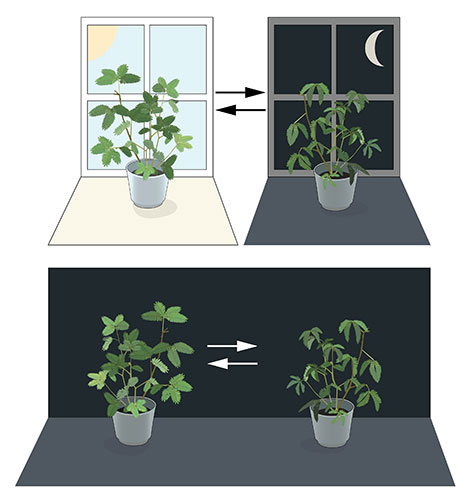
\includegraphics[width=0.5\textwidth,height=\textheight]{qmd/images/nobel-prize-outreach-ab-2017-de-mairan-experiment.png}

\legend{Source: Reproduction from \textcite{nobelprizeoutreachab}.}

}

\end{figure}%

Science has already demonstrated and described various biological
rhythms and their impacts on organisms. These rhythms can occur at
different levels, whether at a macro level, such as the menstrual cycle,
or even at a micro level, such as rhythms expressed within cells
\autocite{roenneberg2016}. Like many other biological phenomena, these
are complex systems present in all living beings, i.e., an emergence
created by a large number of connected and interecticve agents that
exhibit adaptive characteristics, all without the need of a central
control \autocite{boccara2010}. It is understood today that the
endogeneity of rhythms has provided organisms with an anticipatory
capacity, allowing them to organize resources and activities before they
are needed \autocite{marques2003}.

Despite the endogenous nature of these rhythms, they can still be
regulated by the external environment. Signals (cues) from the
environment that occur cyclically and have the ability to regulate
biological rhythmic expression are called zeitgebers (from the German
\emph{zeit}, meaning time, and \emph{geber}, meaning donor
\autocite{cambridgeuniversitypress}). These zeitgebers act as
synchronizers by entraining the phases of biological rhythms
\autocite{khalsa2003,kuhlman2018} (see
Figure~\ref{fig-chapter-2-kuhlman-2018-figure-2b}). Among the known
zeitgebers are, for example, meal timing and changes in environmental
temperature \autocite{aschoff1981,roenneberg2016}. However, the most
influential of them is the light-dark cycle. It is understood that the
day/night cycle, resulting from the rotation of the Earth, has provided
the vast majority of organisms with an oscillatory system with a
periodic duration of approximately 24 hours
\autocite{kuhlman2018,roenneberg2007}.

\begin{figure}[H]

\caption{\label{fig-chapter-2-kuhlman-2018-figure-2b}Illustration of a
circadian rhythm (output) whose phase is entrained in the presence of a
zeitgeber (input). The rectangles represent the light-dark cycle.}

\centering{

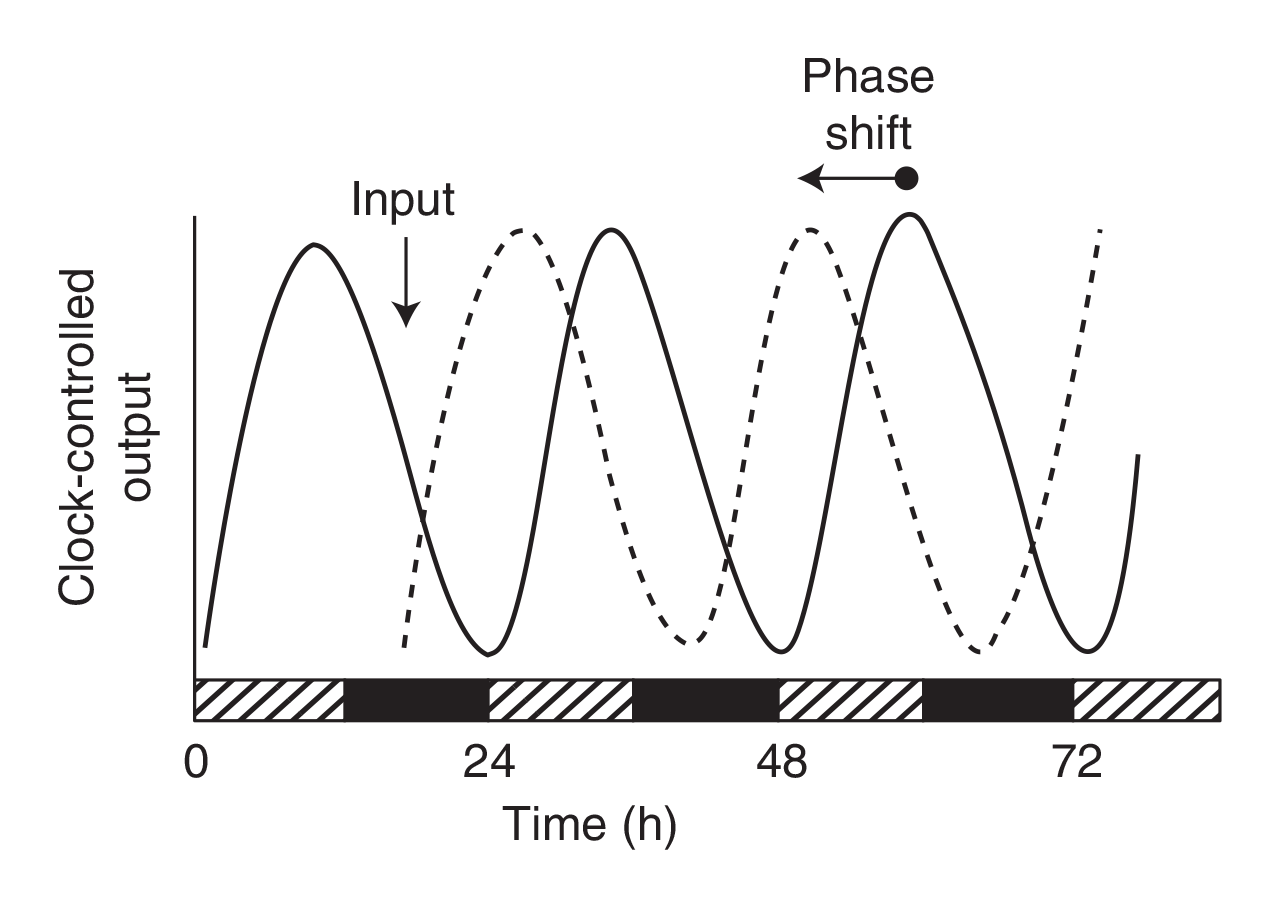
\includegraphics[width=0.75\textwidth,height=\textheight]{qmd/images/kuhlman-2018-figure-2b.png}

\legend{Source: Adapted from \textcite{kuhlman2018}.}

}

\end{figure}%

Naturally, the expression of this temporal organization varies from
organism to organism, even among members of the same species, whether
due to the different ways they are exposed to the environment or the
differences in the expression of endogenous rhythmicity, which, in turn,
results from gene expression \autocite{roenneberg2007a}. The interaction
between these two expressions, external and internal, of the environment
and genotype, generates a signature, an observable characteristic, which
is called a phenotype \autocite{frommlet2016}.

The various temporal characteristics of an organism can be linked to
different oscillatory periods. Among these are circadian phenotypes,
which refer to characteristics observed in rhythms with periods lasting
about a day \autocite{foster2005}. Another term used for these temporal
phenotypes, as the name suggest, is \emph{chronotype}
\autocite{ehret1974,pittendrigh1993}. This term is also often used to
differentiate phenotypes on a spectrum ranging from morningness to
eveningness \autocite{horne1976,roenneberg2019b}.

Sleep is a phenomenon that exhibits circadian expression. By observing
the sleep characteristics of individuals, it is possible to assess the
distribution of circadian phenotypes within a population, thereby
investigating their covariates and other relevant associations
\autocite{roenneberg2003}. This is because sleep regulation is
understood as the result of the interaction between two processes: a
homeostatic process (referred to as the \(\text{S}\) process), which is
sleep-dependent and accumulates with sleep deprivation, and a circadian
process (referred to as the \(\text{C}\) process), whose expression can
be influenced by zeitgebers, such as the light-dark cycle
(Figure~\ref{fig-chapter-2-borbely-1982-figure-4} illustrates these two
process) \autocite{borbely1982,borbely2016}. Considering that the
circadian rhythm (the \(\text{C}\) process) is present in sleep, its
characteristics can be estimated if the \(\text{S}\) process can be
controlled.

\begin{figure}[H]

\caption{\label{fig-chapter-2-borbely-1982-figure-4}Illustration of the
interaction between Process S (sleep-dependent process) and Process C
(circadian rhythm process) in sleep regulation. The figure depicts two
scenarios: one with 17 hours of wakefulness followed by 7 hours of
sleep, and another with sleep deprivation, consisting of 41 hours of
wakefulness followed by 7 hours of sleep. The y-axis represents the
level of each process. The shaded areas indicate periods of sleep, along
with the exponential decline of Process S.}

\centering{

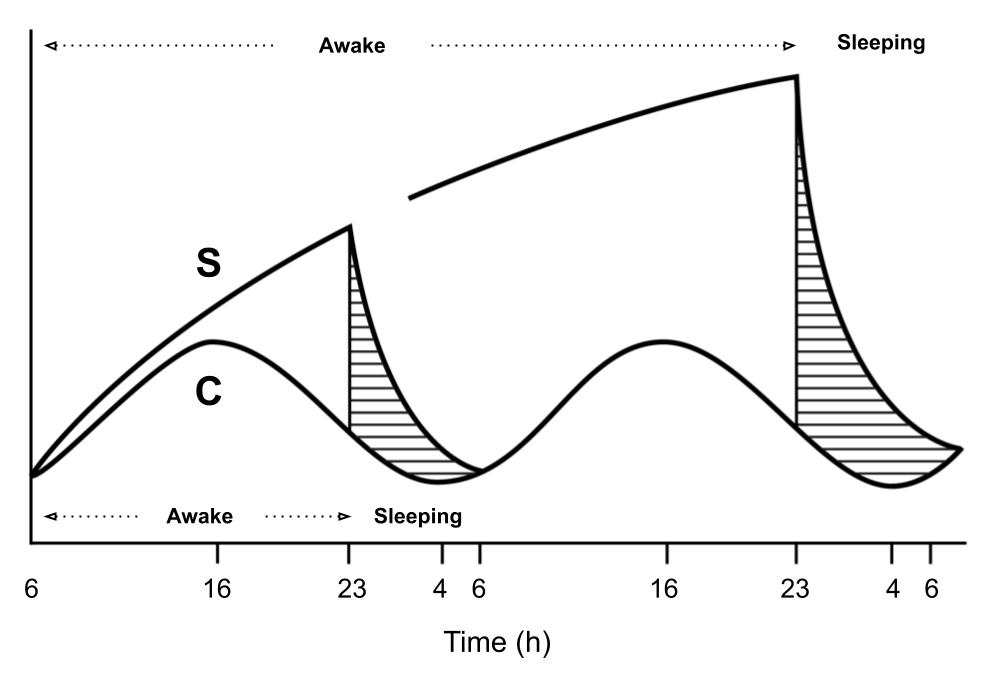
\includegraphics[width=0.75\textwidth,height=\textheight]{qmd/images/borbely-1982-figure-4.png}

\legend{Source: Adapted from \textcite{borbely1982}.}

}

\end{figure}%

{[}Finish explaining about the MCTQ and its proxy for the chronotype{]}

\bookmarksetup{startatroot}

\chapter{On complexity science}\label{on-complexity-science}

\begin{tcolorbox}[enhanced jigsaw, opacitybacktitle=0.6, titlerule=0mm, coltitle=black, bottomtitle=1mm, breakable, rightrule=.15mm, left=2mm, title=\textcolor{quarto-callout-important-color}{\faExclamation}\hspace{0.5em}{Important}, opacityback=0, colbacktitle=quarto-callout-important-color!10!white, toprule=.15mm, toptitle=1mm, leftrule=.75mm, colback=white, bottomrule=.15mm, arc=.35mm, colframe=quarto-callout-important-color-frame]

You are reading the work-in-progress of this thesis.

\microskip

This chapter is currently a dumping ground for ideas, and I don't
recommend reading it.

\end{tcolorbox}

Complex versus Complicated.

\textbf{Complex systems} are systems with many interconnected parts that
exhibit emergent behavior.

\textbf{Stable macroscopic patterns} arising from \textbf{local
interaction} of agents \autocite{epstein1999}.

In mathematical terms, the interactions of interest are non-linear
\autocite{holland2014}.

When the aggregate exhibits \textbf{properties not attained by
summation} \autocite{holland2014}.

The behavior of each part don't explain how they behave collectively.

Emergence: new properties that arise from the interactions of the parts
of a system, which are not present in the parts themselves. Collective
behavior. Aggregate behavior.

You are dealing with an emergence phenomenon when there is no need to
look under the hood \autocite{krakauer2023}.

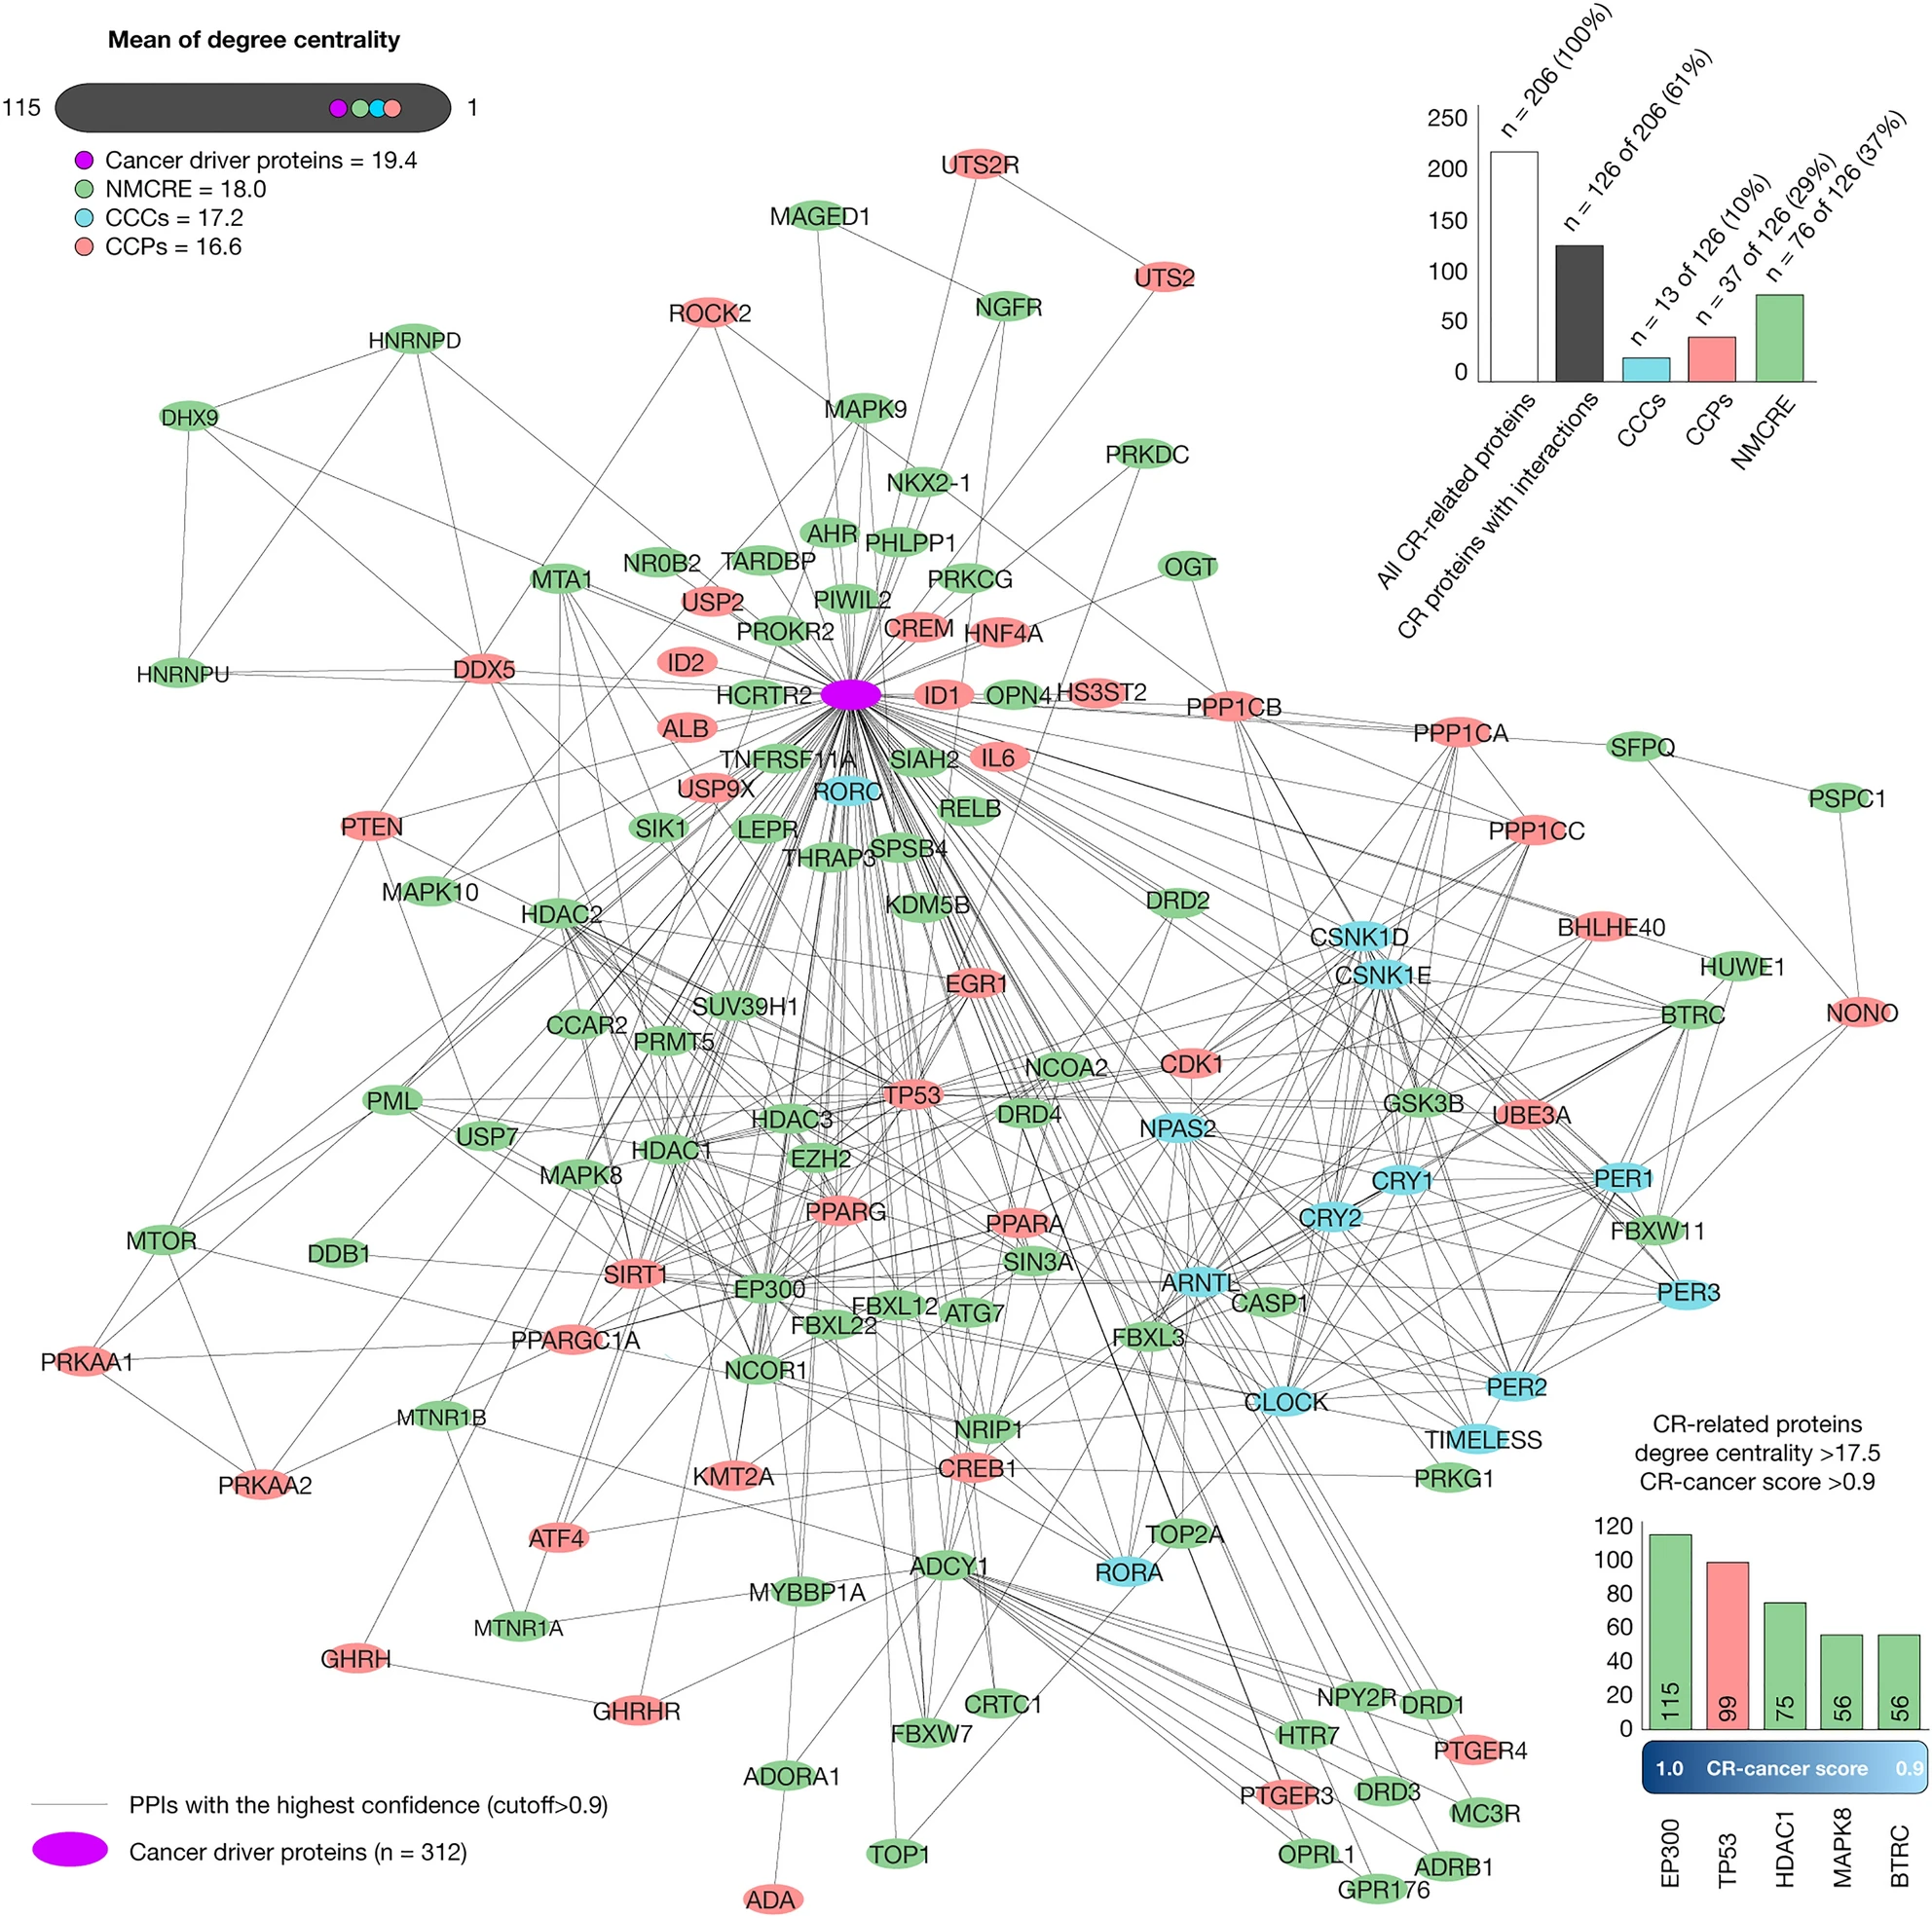
\includegraphics{qmd/images/perez-villa-2023-figure-3.png}

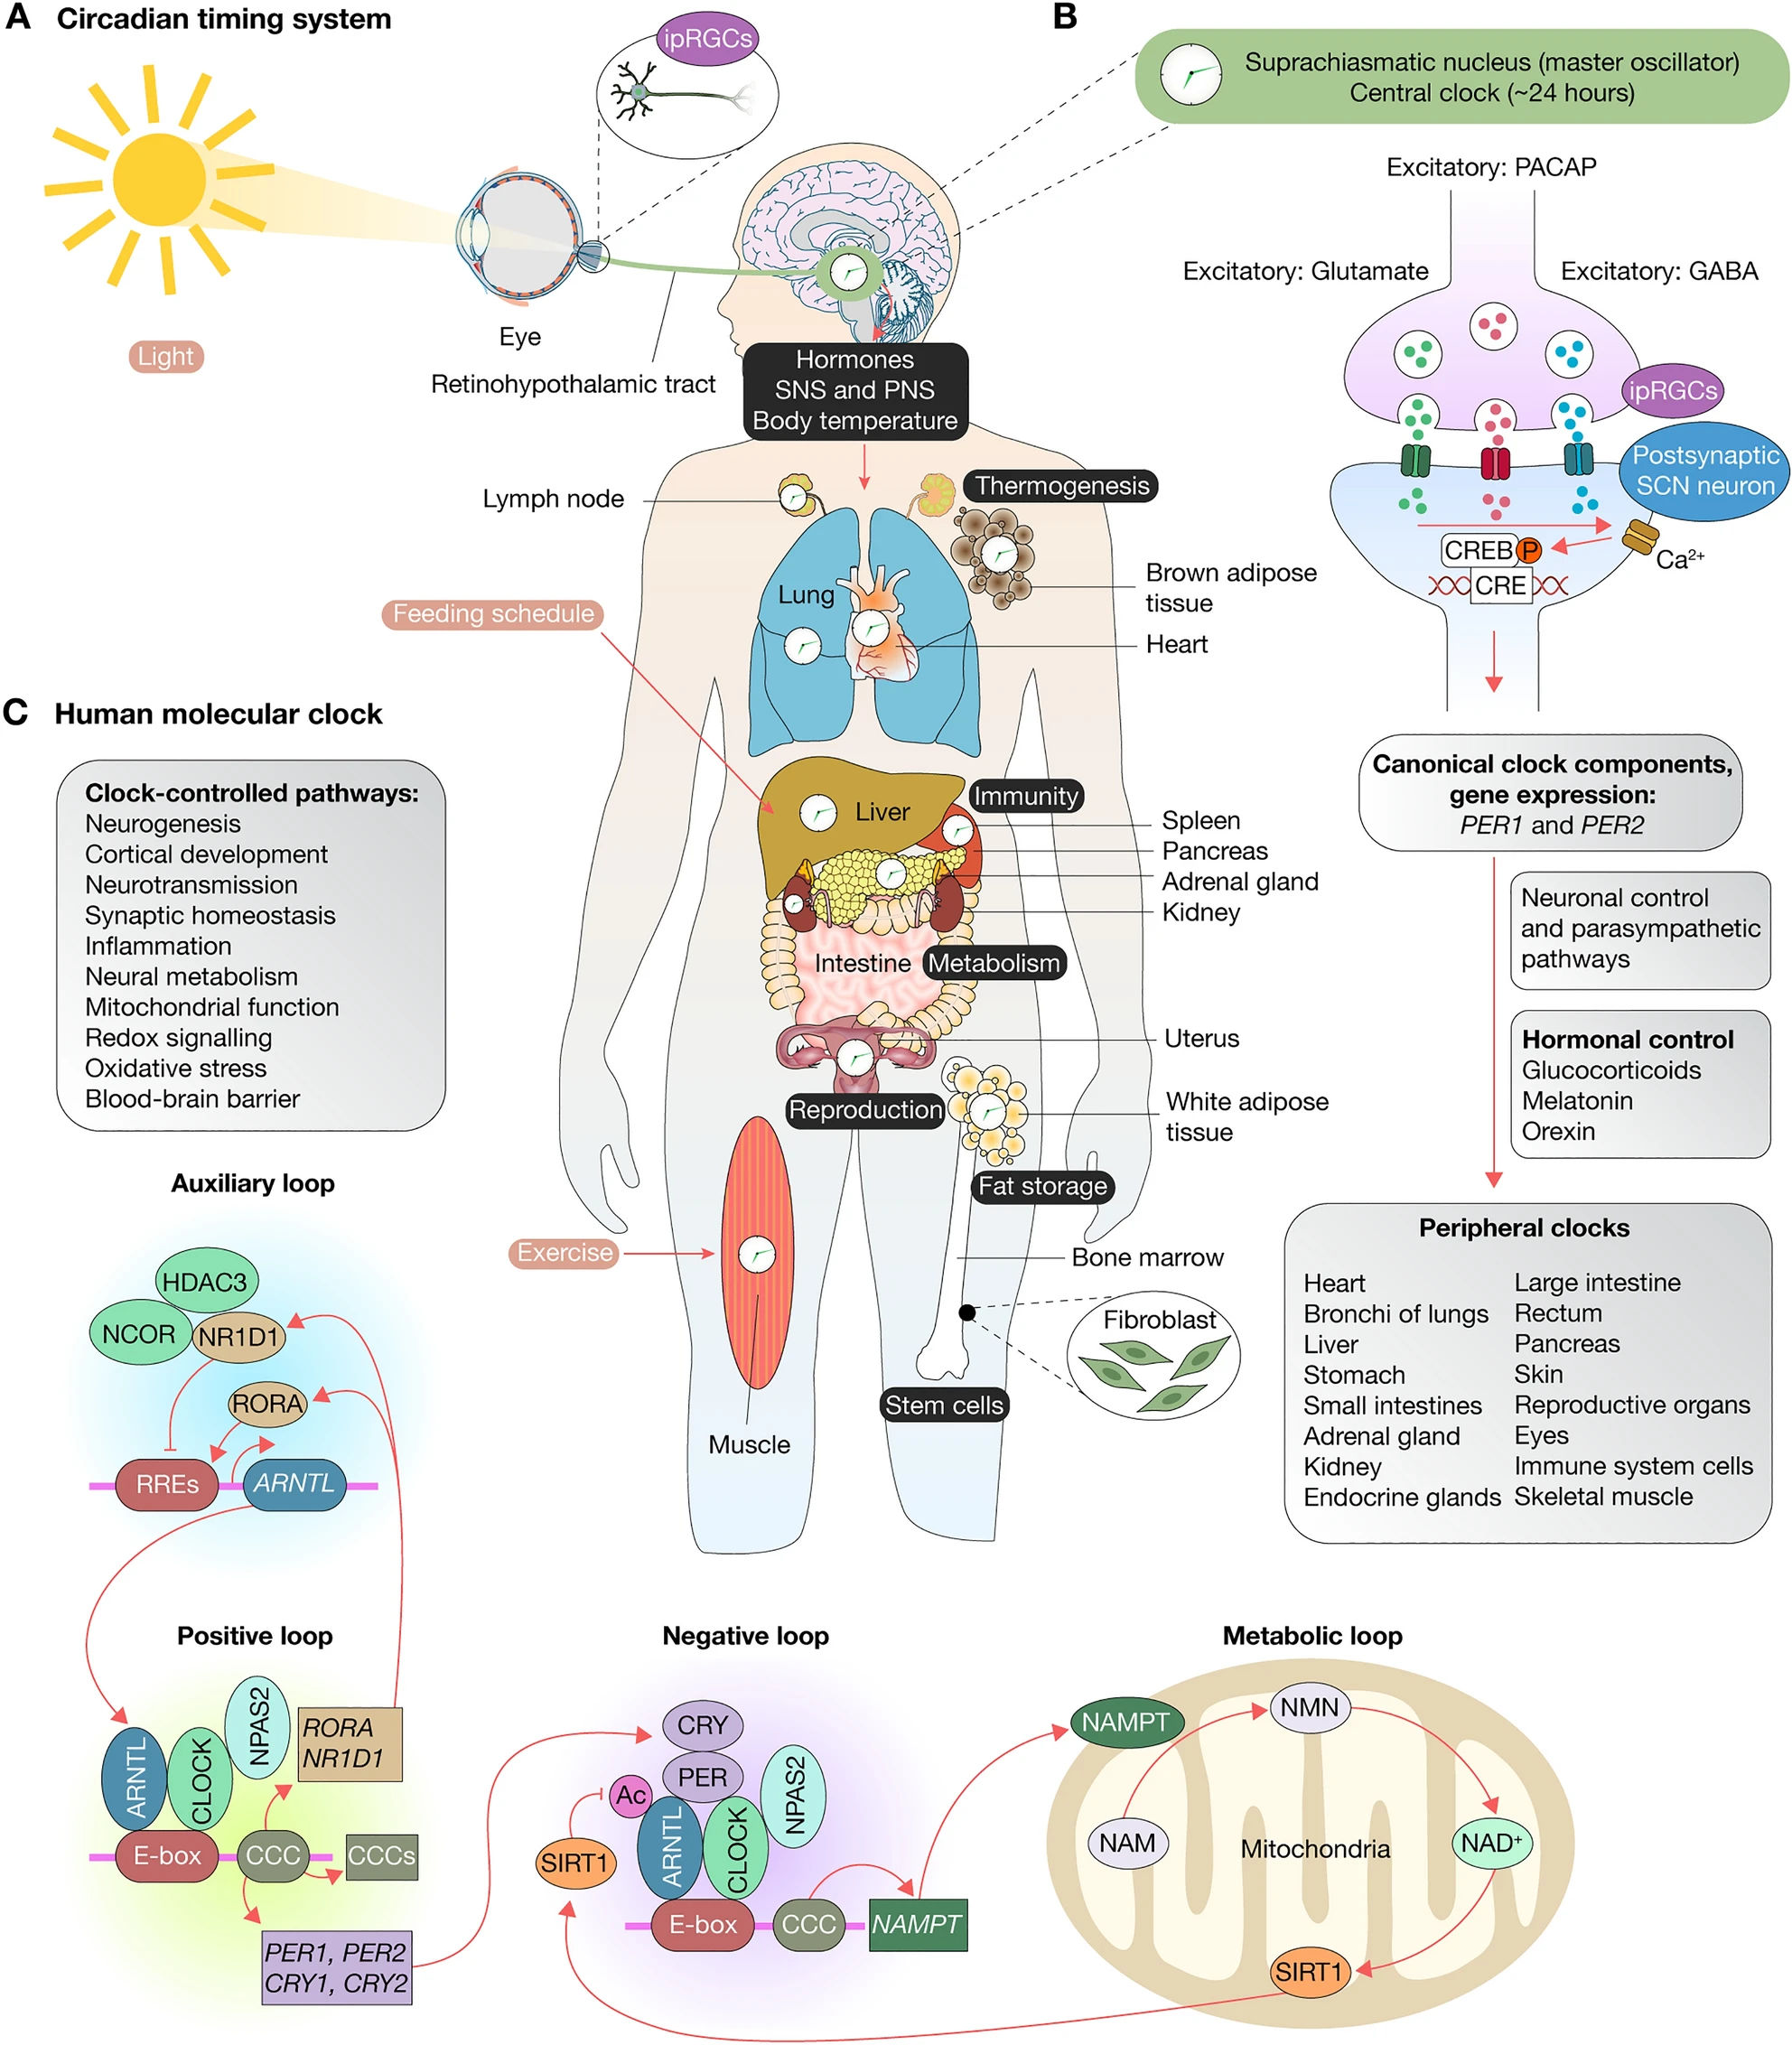
\includegraphics{qmd/images/perez-villa-2023-figure-1.png}

The result of a \emph{juggling act} of billions of years of evolution.
There are no specific functions. There's no proposed goal.

Levels of description \autocite{nicolis2012}. Starting in the cell
nucleus with the molecular clock, then the cell, the tissue, the organ
following to stable macroscopic patterns of circadian rhythms in
behavior and physiology.

If you think about it, the extensive clock control is like a
finely-tuned choreography. Everything is organized to happen at the
right time, just like a \textbf{Rube Goldberg machine}
\autocite{merrow2020}.

Circadian clocks regulate and/or modulate functions at all levels,
ranging from gene expression and physiology to behavior and cogitation
\autocite{roenneberg2007}.

It's an emergent phenomenon. It's not a property of the parts
themselves. It's a property of the system as a whole.

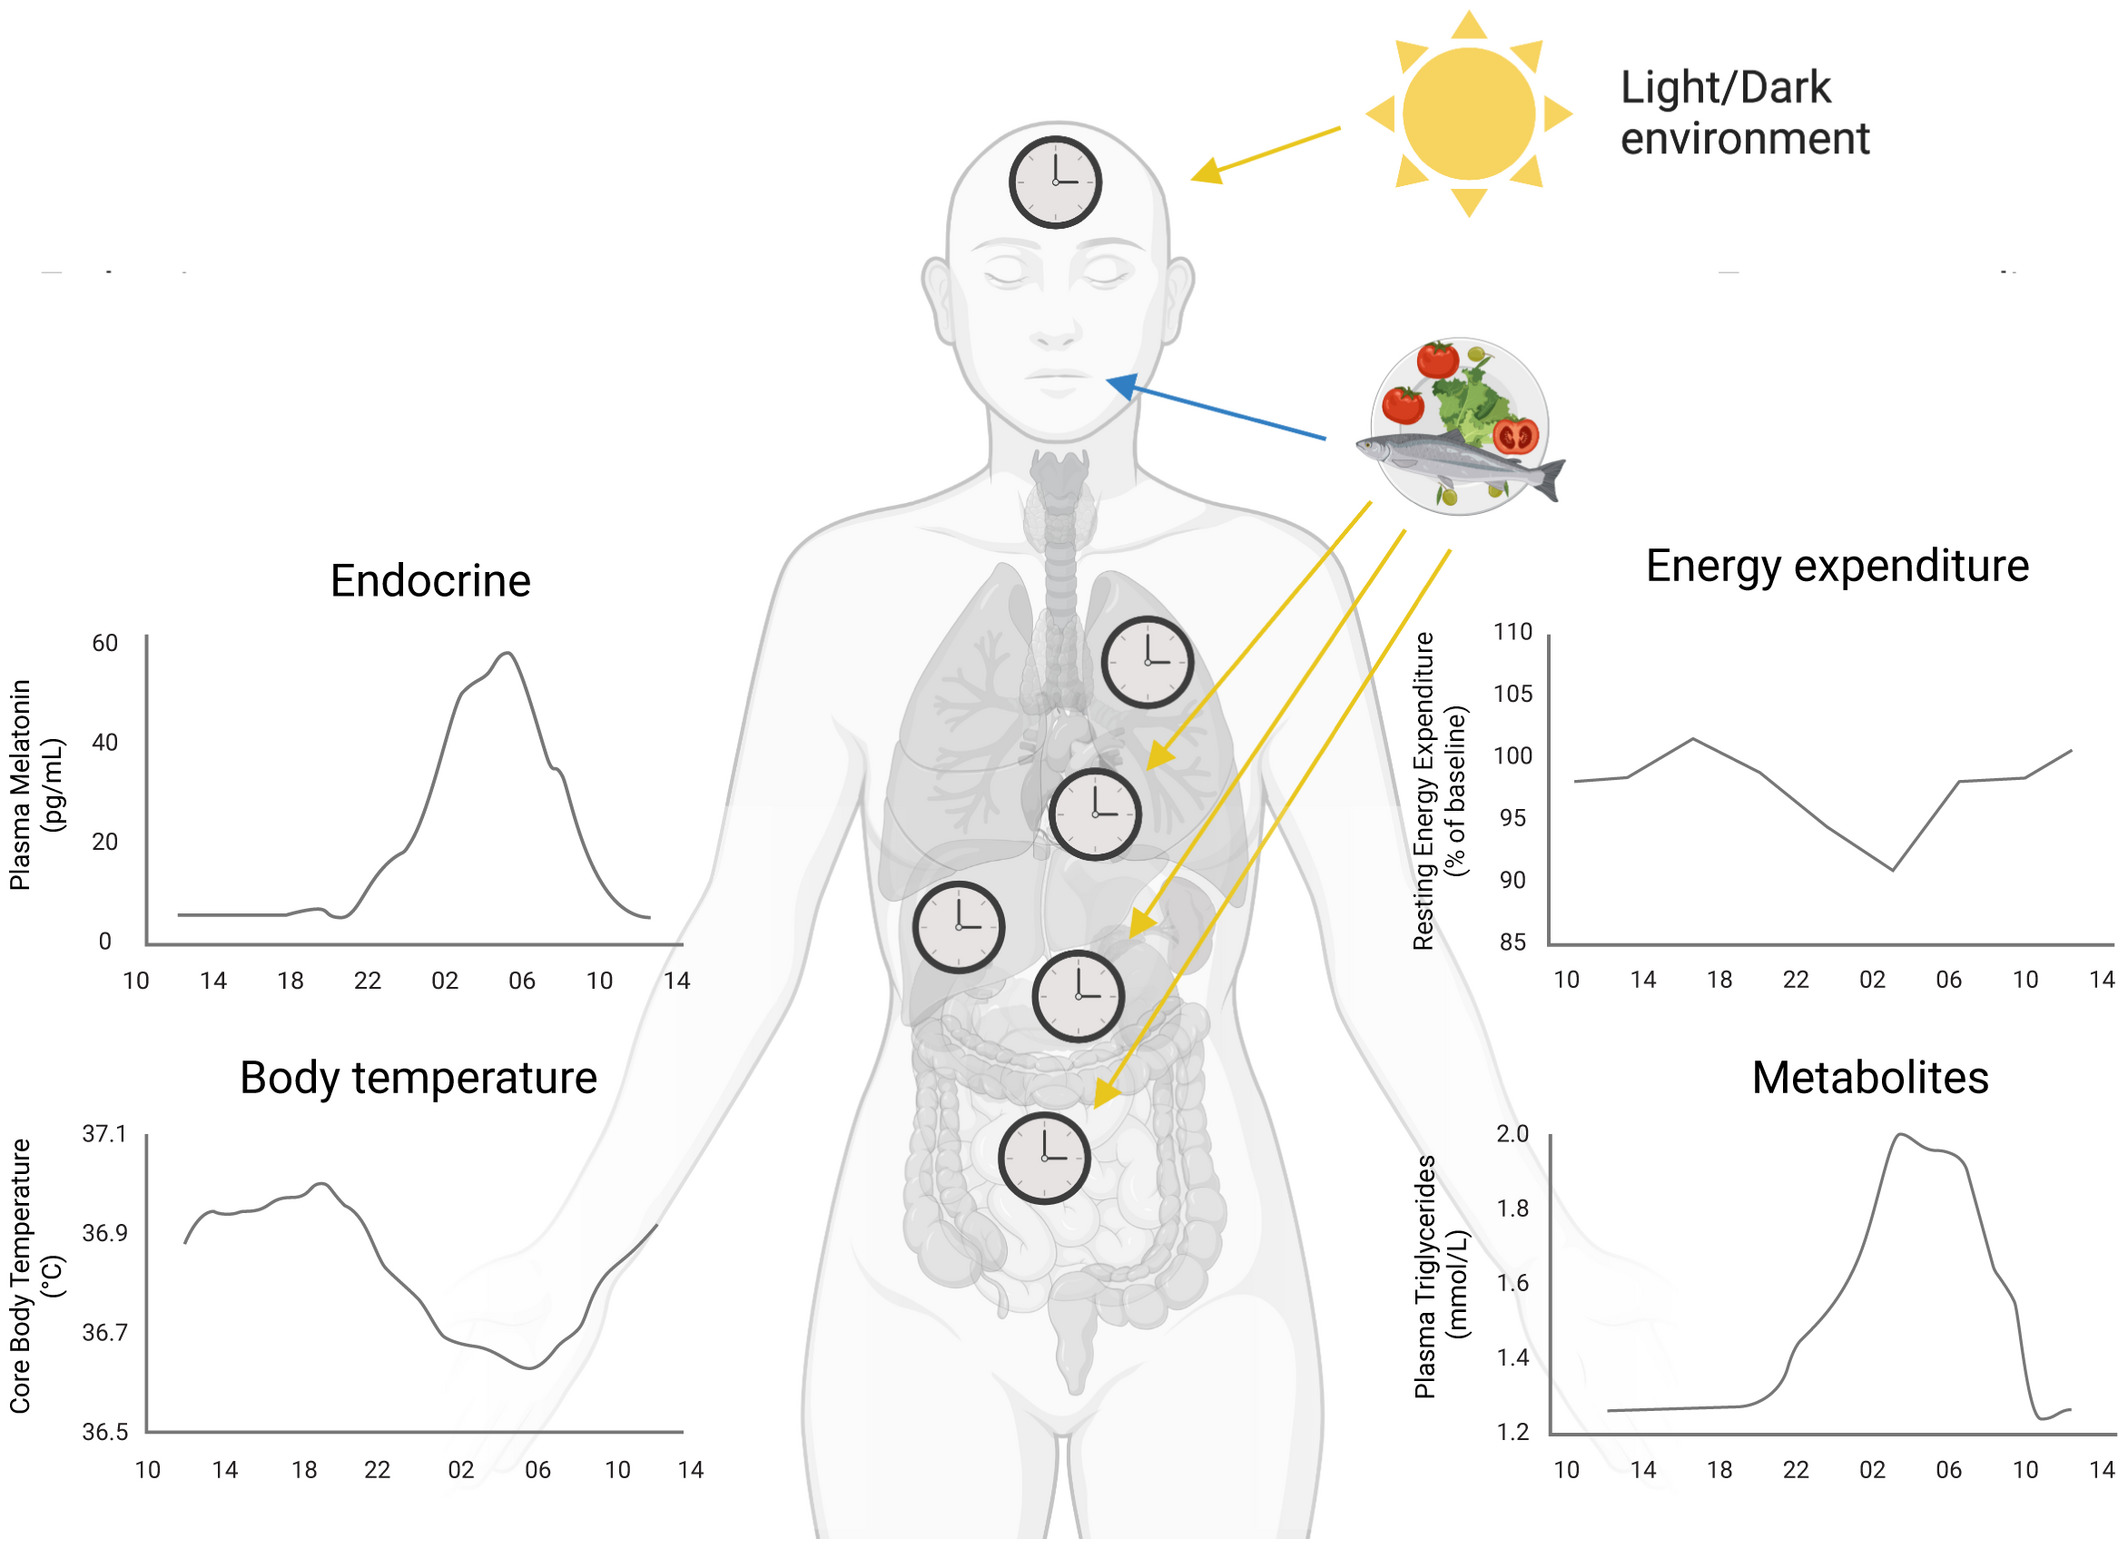
\includegraphics{qmd/images/flanagan-2021-figure-2.png}

``{[}\ldots{]} involve great numbers of parts undergoing a kaleidoscopic
array of simultaneous interactions.'' \autocite{holland1992b}

In complex adaptive systems, \textbf{emergent properties} often occur
when coevolving signals and boundaries generate \textbf{new levels of
organization} \autocite{holland2012}.

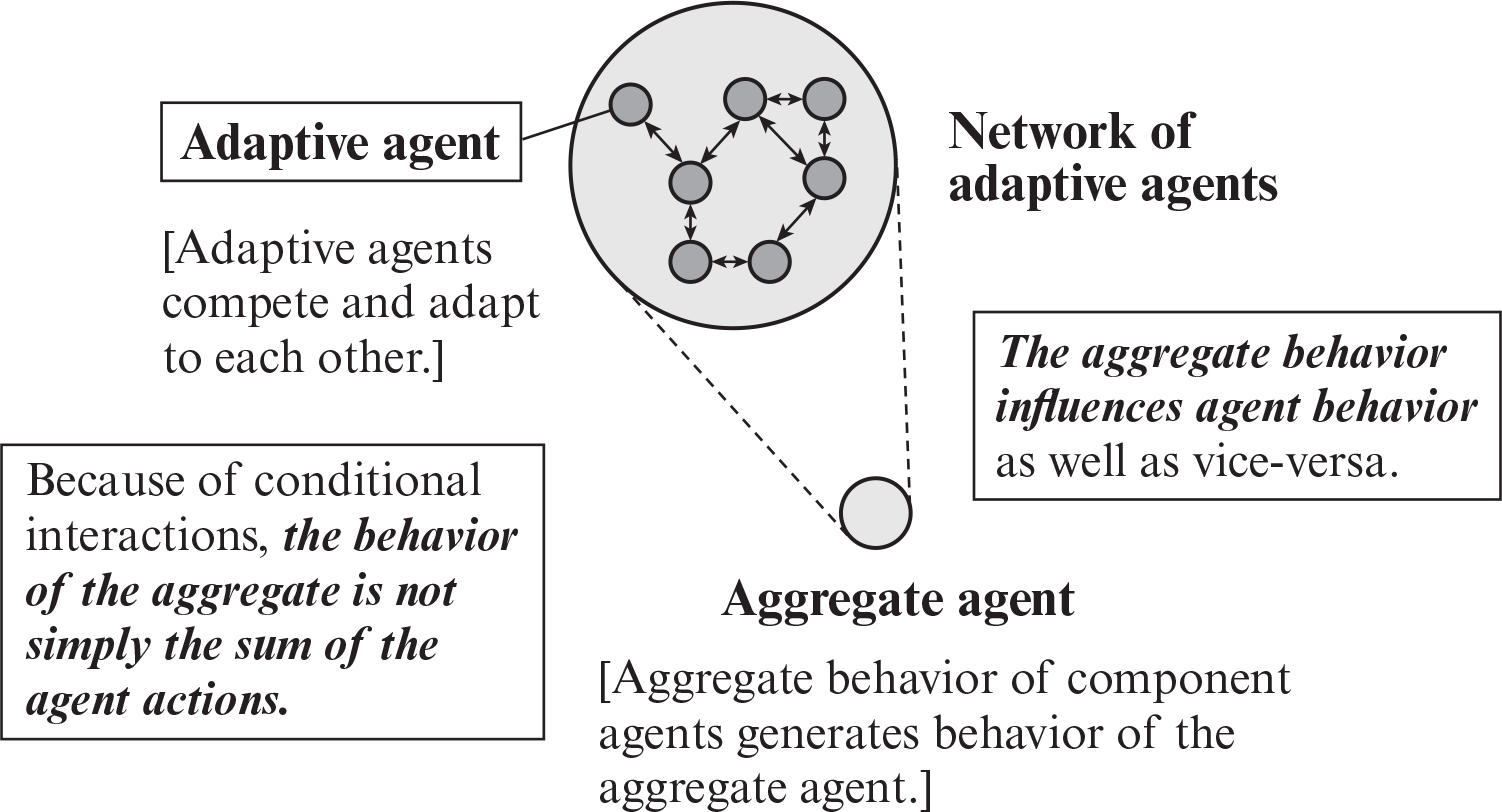
\includegraphics{qmd/images/holland-2012-figure-1.png}

Structural levels

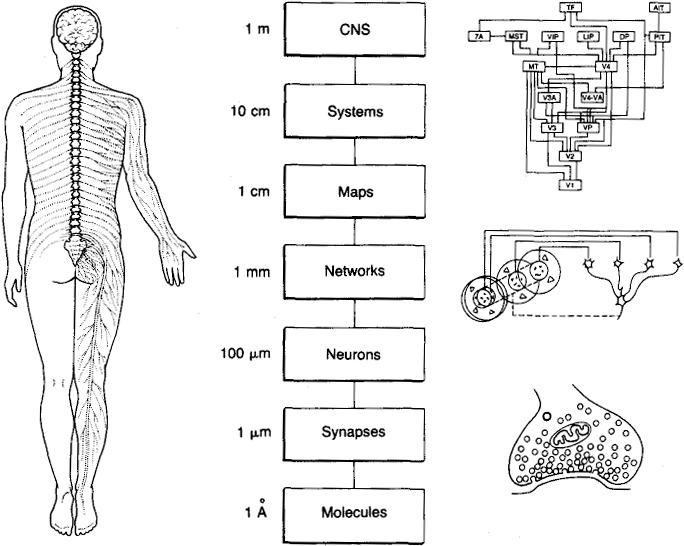
\includegraphics{qmd/images/lewin-1993-figure-8.png}

Fig. 8. Structural levels in the organization of the nervous system, a
reflection of the hierarchical systems that may underlie the generation
of higher cognitive functions, including consciousness. Courtesy of
Patricia Churchland and Terrence Sejnowski.

A system of many interacting parts where the system is \textbf{more than
just the sum of its parts} (Mark Newman in \textcite{mitchell2013}).

A system that involves a large number of parts undergoing a
kaleidoscopic array of simultaneous interactions, exhibiting
\textbf{aggregate behavior} that cannot be simply derived from the
actions of the individual parts \autocite{holland1992b}.

Systems with many connected agents that interact and exhibit
self-organization and \textbf{emergence behavior}, all without the need
for a central controller (Camilo Rodrigues Neto).

Dialectics at its finest (my working definition).

Complexity science seeks to \textbf{explain emergent phenomena} or
mechanisms that ``screen-off'' their constituent parts and thereby allow
new levels of description and understanding \autocite{krakauer2024}.

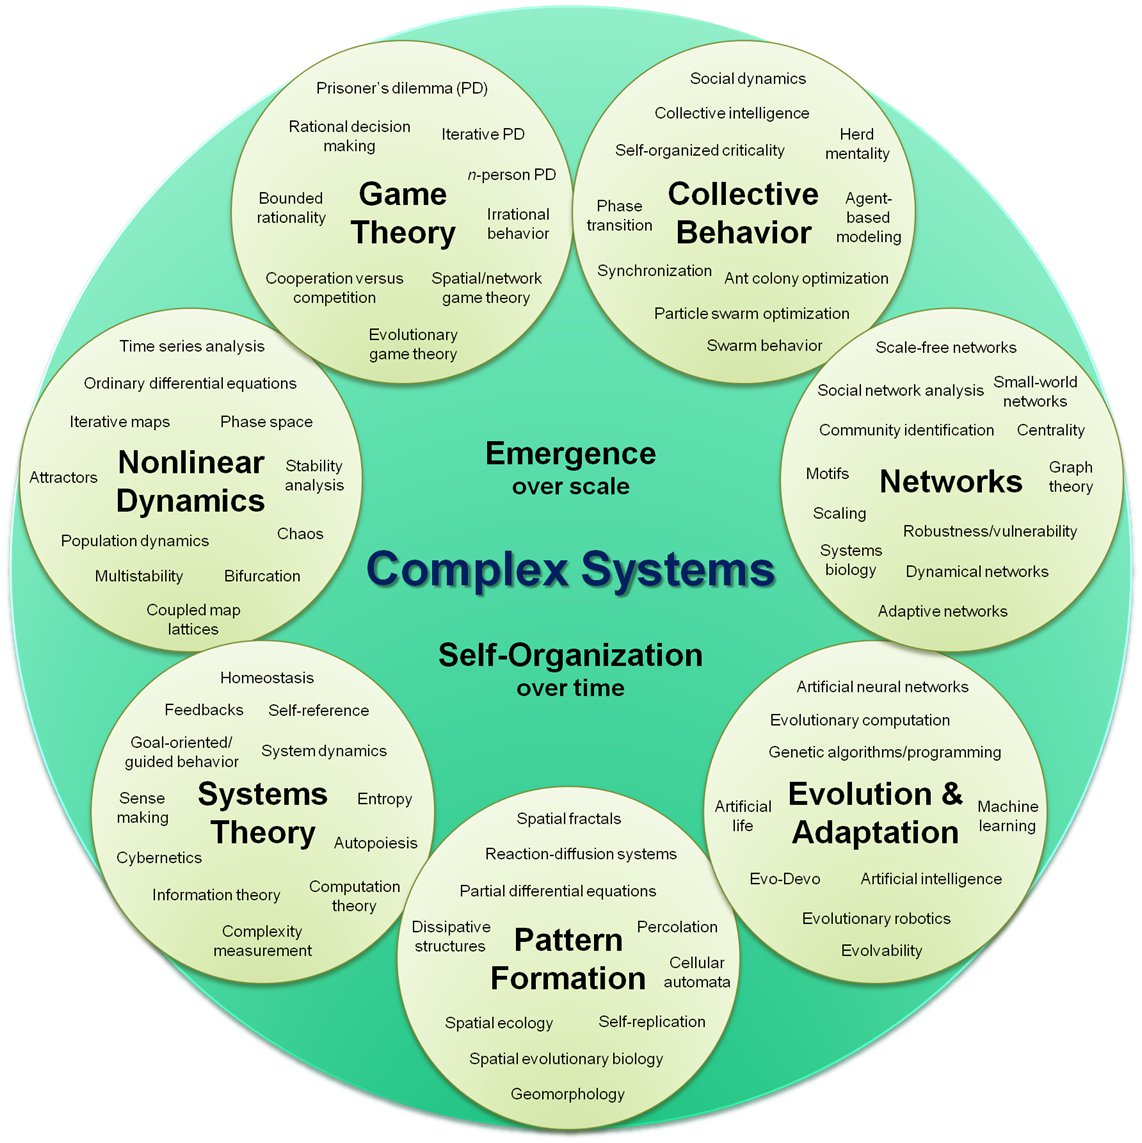
\includegraphics{qmd/images/sayama-2015-figure-1.png}

The seven basics consist of 4 properties and 3 mechanisms that are
common to all complex adaptive systems:

\begin{itemize}
\tightlist
\item
  Aggregation (property)
\item
  Nonlinearity (property)
\item
  Flows (property)
\item
  Diversity (property)
\item
  Tags (mechanism)
\item
  Internal models (mechanism)
\item
  Building blocks (mechanism)
\end{itemize}

\autocite{holland1996}

Other concepts: chaos, power laws \& factor sparsity, feedback loops,
robustness, equilibrium states, path dependence, leverage points

Approaches to study and model circadian clocks.

\bookmarksetup{startatroot}

\chapter{On the latitude hypothesis}\label{on-the-latitude-hypothesis}

\begin{tcolorbox}[enhanced jigsaw, opacitybacktitle=0.6, titlerule=0mm, coltitle=black, bottomtitle=1mm, breakable, rightrule=.15mm, left=2mm, title=\textcolor{quarto-callout-important-color}{\faExclamation}\hspace{0.5em}{Important}, opacityback=0, colbacktitle=quarto-callout-important-color!10!white, toprule=.15mm, toptitle=1mm, leftrule=.75mm, colback=white, bottomrule=.15mm, arc=.35mm, colframe=quarto-callout-important-color-frame]

You are reading the work-in-progress of this thesis.

\microskip

This chapter is currently a dumping ground for ideas, and I don't
recommend reading it.

\end{tcolorbox}

Although many theories related to sleep and circadian rhythms are
well-established in science, it is still necessary to verify and test
them in larger samples to obtain a more accurate picture of the
mechanisms related to the ecology of sleep and chronotypes. This project
undertakes this commitment with the aim of investigating a hypothesis
that is still relatively untested but widely accepted in chronobiology,
which suggests that latitude is associated with the regulation of
circadian rhythms
\autocite{hut2013,leocadio-miguel2014,leocadio-miguel2017,pittendrigh1991,randler2008,randler2017,roenneberg2003}.

The latitude hypothesis is based on the idea that regions located at
latitudes close to the poles, on average, experience less annual
sunlight exposure compared to regions near the equator. Therefore, it is
deduced that regions near latitude 0° have a stronger solar zeitgeber,
which, according to chronobiology theories, should lead to a greater
propensity for the synchronization of circadian rhythms in these
populations with the light-dark cycle. This would reduce the amplitude
and diversity of circadian phenotypes found due to a lower influence of
individuals' characteristic endogenous periods
(Figure~\ref{fig-chapter-2-roenneberg-2003-figure-7-f} illustrates this
effect). This would also give these populations a morningness
characteristic when compared to populations living farther from the
equator, where the opposite would occur -- greater amplitude and
diversity of circadian phenotypes and an eveningness characteristic
compared to populations living near latitude 0°
\autocite{roenneberg2003}.

\begin{figure}[H]

\caption{\label{fig-chapter-2-roenneberg-2003-figure-7-f}Different
chronotype distributions, influenced by strong and weak zeitgebers --
black for strong and hatched for weak. An illustration of the effect
hypothesized by the latitude hypothesis.}

\centering{

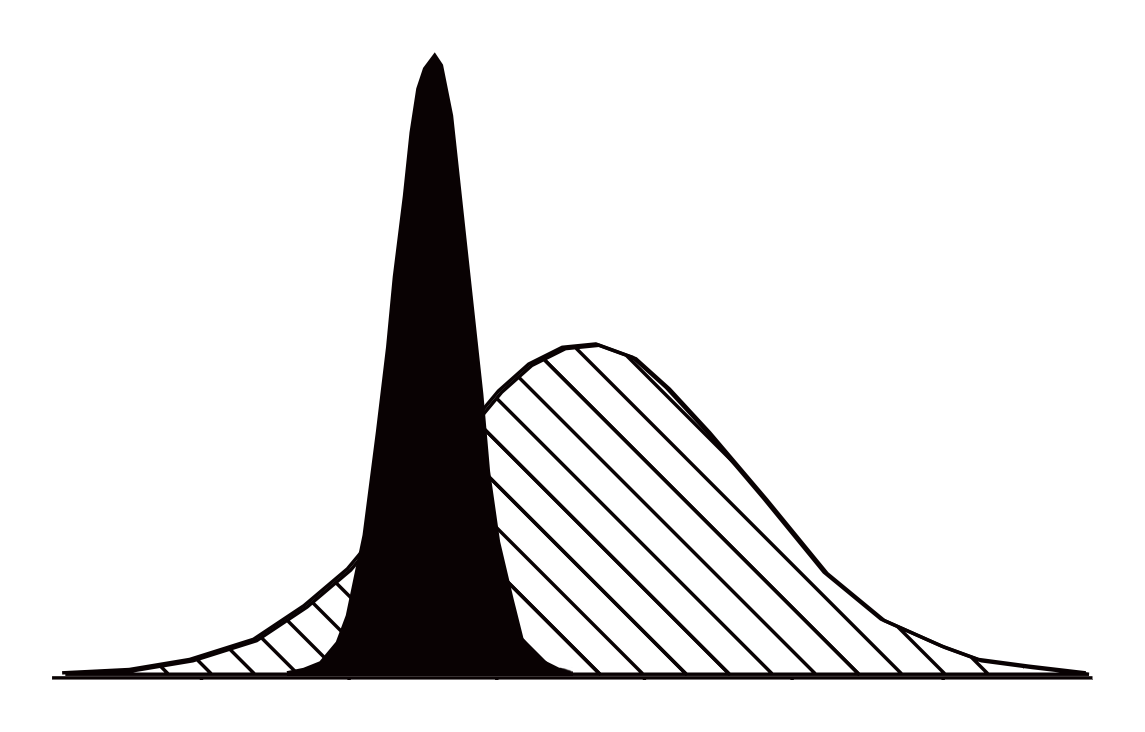
\includegraphics[width=0.75\textwidth,height=\textheight]{qmd/images/roenneberg-2003-figure-7-f.png}

\legend{Source: Adapted from \textcite{roenneberg2003}.}

}

\end{figure}%

``However, it is also our experience that some mathematically
sophisticated scientists may lack the conceptual frame that links the
mathematical procedures to the substantive scientific task in a
particular case'' \autocite{cohen2002}.

Effect sizes. Statistical ritual versus statistical thinking
\autocite{gigerenzer2004}.

A p-value is not evidence of the existence of an effect., it's only
indirect evidence at best. Large samples and the p-value problem
\autocite{lin2013}. P-values as an exponential model of data sizes
\autocite{mariscal2021}. A small p-value does not imply that there is an
important effect; it only tells us something about the plausibility of
the effect. You need to have a meaningful effect to have an interesting
result, and the p-value doesn't tell you that.

Confidence intervals for an effect size measure in multiple linear
regression \autocite{algina2007}. Setting hypotheses with effect sizes:
minimal effect size \autocite{perezgonzalez2015}.

The original article had two issues regarding data testing, commonly
related to null hypothesis significance tests (NHST). It is not within
the scope of this article to discuss all the issues regarding NHST; for
that, I recommend checking \textcite{perezgonzalez2015}. The two main
methodological issues regarding the hypothesis test in the original
article were:

\begin{enumerate}
\def\labelenumi{\arabic{enumi}.}
\tightlist
\item
  Using the p-value instead of the effect size as a criterion for
  rejecting or accepting the alternative hypothesis;
\item
  Failing to integrate a minimum effect size in the alternative
  hypothesis. A test without the latter can create serious distortions
  in the interpretation of the results, since even a negligible effect
  could lead to the acceptance of the alternative hypothesis.
\end{enumerate}

Considering the particular emphasis that the solar zeitgeber has on the
entrainment of biological rhythms (as demonstrated in many experiments),
it would not be reasonable to assume that the latitude hypothesis could
be supported without at least a non-negligible effect size. Although the
latitude association claimed by many authors implies not just a linear
relationship but also a significant effect on chronotype, considering
the biological construct of chronotype, the approach that incorporates a
minimum effect size (MES) is not new. In fact, when Neyman and Pearson
published their schema for data testing, a MES was required.

Even assuming a very low threshold, similar to the claim of 2\% variance
explained by latitude as a predictor, the hypothesis does not hold. As
shown by \textcite{leocadio-miguel2017}, adding \(0.00388\) to the
\(\text{R}^2\) results in Cohen's
\(f^2 = (0.06352 - 0.05964) / (1 - 0.06352) = 0.004143174\), which is
negligible by all standards. Again, the conclusion drawn by the authors
of this study was not based on sound statistical thinking.

y-axis illusion. unbalanced data.

\bookmarksetup{startatroot}

\chapter{Is latitude associated with
chronotype?}\label{is-latitude-associated-with-chronotype}

\begin{tcolorbox}[enhanced jigsaw, opacitybacktitle=0.6, titlerule=0mm, coltitle=black, bottomtitle=1mm, breakable, rightrule=.15mm, left=2mm, title=\textcolor{quarto-callout-note-color}{\faInfo}\hspace{0.5em}{Note}, opacityback=0, colbacktitle=quarto-callout-note-color!10!white, toprule=.15mm, toptitle=1mm, leftrule=.75mm, colback=white, bottomrule=.15mm, arc=.35mm, colframe=quarto-callout-note-color-frame]

You are reading the work-in-progress of this thesis.

\microskip

This chapter should be readable but is currently undergoing final
polishing.

\end{tcolorbox}

\begin{tcolorbox}[enhanced jigsaw, opacitybacktitle=0.6, titlerule=0mm, coltitle=black, bottomtitle=1mm, breakable, rightrule=.15mm, left=2mm, title=\textcolor{quarto-callout-warning-color}{\faExclamationTriangle}\hspace{0.5em}{Warning}, opacityback=0, colbacktitle=quarto-callout-warning-color!10!white, toprule=.15mm, toptitle=1mm, leftrule=.75mm, colback=white, bottomrule=.15mm, arc=.35mm, colframe=quarto-callout-warning-color-frame]

The results shown here are \textbf{preliminary}, so please take them
with a grain of salt.

\microskip

The data has not yet been fully cleaned, balanced, and cross-referenced
with the secondary databases. Think of these results as a low-resolution
preview of the final results. The step-by-step analysis can be seen in
the appendices section.

\end{tcolorbox}

\begin{tcolorbox}[enhanced jigsaw, opacitybacktitle=0.6, titlerule=0mm, coltitle=black, bottomtitle=1mm, breakable, rightrule=.15mm, left=2mm, title=\textcolor{quarto-callout-note-color}{\faInfo}\hspace{0.5em}{Target journal}, opacityback=0, colbacktitle=quarto-callout-note-color!10!white, toprule=.15mm, toptitle=1mm, leftrule=.75mm, colback=white, bottomrule=.15mm, arc=.35mm, colframe=quarto-callout-note-color-frame]

\begin{enumerate}
\def\labelenumi{\arabic{enumi}.}
\tightlist
\item
  \href{https://www.nature.com/srep/author-instructions}{Scientific
  Reports} (\href{https://jcr.clarivate.com/jcr/}{IF 2022: 4.6/JCR}
  \textbar{}
  \href{https://sucupira.capes.gov.br/sucupira/public/consultas/coleta/veiculoPublicacaoQualis/listaConsultaGeralPeriodicos.jsf}{A1/2017-2020}).
\end{enumerate}

\end{tcolorbox}

\begin{tcolorbox}[enhanced jigsaw, opacitybacktitle=0.6, titlerule=0mm, coltitle=black, bottomtitle=1mm, breakable, rightrule=.15mm, left=2mm, title=\textcolor{quarto-callout-note-color}{\faInfo}\hspace{0.5em}{Note}, opacityback=0, colbacktitle=quarto-callout-note-color!10!white, toprule=.15mm, toptitle=1mm, leftrule=.75mm, colback=white, bottomrule=.15mm, arc=.35mm, colframe=quarto-callout-note-color-frame]

The following study was performed by Daniel Vartanian (DV), Mario
Pedrazzoli (MP) and Camilo Rodrigues Neto (CR).

\microskip

\textbf{DV} contributed to the design and implementation of the study.
\textbf{DV} and \textbf{MP} collected the data. \textbf{DV} and
\textbf{CR} performed the statistical analysis. \textbf{DV} wrote the
manuscript. All authors discussed the results and revised the final
manuscript.

\microskip

\emph{Future reference}: Vartanian, D., Pedrazzoli, M., \& Rodrigues
Neto, C. (2024). A biological approach for the latitudinal cline of the
chronotype. \emph{Scientific Reports}.

\end{tcolorbox}

\noindent \textbf{Chronotypes are temporal phenotypes
\autocite{ehret1974,pittendrigh1993}. Observable traits, like weight and
eye color. Our current understanding of these traits is that they are
linked to our environment and are the result of evolution pressures for
creating an inner temporal organization
\autocite{aschoff1989,paranjpe2005}, a way that organisms found to
anticipate events. Having such an important function in nature, these
internal rhythms need to be closely aligned with environmental changes.
The agents that shift these oscillations towards the environment are
called zeitgebers and the shift phenomenon is called entrainment
\autocite{roenneberg2003a,roenneberg2010}. The main zeitgeber for humans
is light exposure, particularly the light of the sun
\autocite{khalsa2003,minors1991,roenneberg2007a}. Considering the major
role of light on entrainment, several studies hypothesized that the
latitude shift of the sun could influence or even define the chronotypes
of different populations
\autocite{horzum2015,hut2013,leocadio-miguel2017,leocadio-miguel2014,pittendrigh1991,randler2017}.
For example, populations that live close to the equator would be, on
average, more entrained to the light-dark cycle and have morning-leaning
characteristics. Here we test this hypothesis using a biological
measure, the chronotype state, provided by the Munich ChronoType
Questionnaire \autocite{roenneberg2003}. We tested the latitude
hypothesis on a sample with \(76,744\) subjects living in different
latitudes in Brazil. Our results show that, even with a wide, big, and
aligned sample, the latitude is associated only with negligible effect
sizes. The entrainment phenomenon appears to be much more complex than
previously imagined, opening new questions and contradictions that need
to be further investigated.}

\section{Main text}\label{main-text}

\subsection{Introduction}\label{introduction-1}

Humans can differ from one another in many ways. These observable
traits, like hair color or height, are called phenotypes and are also
presented in the way that our body functions.

A chronotype is a temporal phenotype
\autocite{ehret1974,pittendrigh1993}. This word is usually used to refer
to endogenous circadian rhythms, i.e., rhythms which periods that are
close to a day or 24 hours (\emph{circa diem}). The current body of
knowledge of Chronobiology, the science that studies biological rhythms,
indicates that the evolution of these internal oscillators is linked to
our oscillatory environment, like the day and night cycle, which, along
with our evolution, created environmental pressures for the development
of a temporal organization \autocite{aschoff1989,paranjpe2005}. A way in
which an organism could predict events and better manage its needs, like
storing food for the winter.

A temporal system wouldn't be of much use if it could not follow
environmental changes. To those environmental signals that can regulate
the biological rhythms are given the name zeitgeber (from the German
Zeit, time, and Geber, giver). These zeitgebers produce inputs in our
bodies that can shift and align those rhythms. This phenomenon is called
entrainment \autocite{roenneberg2003a,roenneberg2010}.

The main zeitgeber known today is the light, particularly the sun's
light \autocite{khalsa2003,minors1991,roenneberg2007a}. Considering its
influence in entraining the biological temporal system, several studies
hypothesize that the latitudinal shift of the sun, related to the
earth's axis, would produce, on average, different temporal traits in
populations that live close to the equator line when compared to
populations that live close to the planet's poles
\autocite{horzum2015,hut2013,leocadio-miguel2017,leocadio-miguel2014,pittendrigh1991,randler2017}.
That is because the latter ones would have greater oscillations in sun
activity and an overall weak solar zeitgeber. This is the latitude
hypothesis, that can also appear as the environmental hypothesis of
circadian rhythm regulation.

Recently there have been attempts to test the latitude hypothesis in
different settings, but, at least in humans, none of them have been
successful in seeing a significant effect size related to the
latitudinal cline. Some of these approaches worked with secondary data
and with small samples. One of the most serious attempts of testing this
hypothesis was made by Leocadio-Miguel et al.
\autocite*{leocadio-miguel2017}. They measured the chronotype of
\(12,884\) Brazillian subjects on a wide latitudinal spectrum using the
Morningness--Eveningness Questionnaire (MEQ). Their results showed a
negligible effect size. One possible reason for this is that the MEQ
measures psychological traits and not biological states
\autocite{roenneberg2019}, i.e., the circadian oscillation itself,
therefore, it's not the best way to answer the question
\autocite{leocadio-miguel2014}.

This article brings a novel attempt to test the latitude hypothesis,
using, this time, a biological approach provided by the Munich
ChronoType Questionnaire (MCTQ) \autocite{roenneberg2003}. Furthermore,
the test was carried out on the biggest chronotype sample ever collected
in a same country. A sample made of \(76,744\) subjects, all living in
the same timezone in Brazil, with only one week of difference between
questionnaire responses.

\subsection{Results}\label{results}

The local time of the sleep corrected midpoint between sleep onset and
sleep end on work-free days (MSF\textsubscript{sc}), MCTQ proxy for
measuring the chronotype, had an overall mean of \(\text{04:28:35}\).
The distribution curve is shown in
Figure~\ref{fig-chapter-5-chronotype-distribution}.

That's the midsleep point of Brazilian subjects with an
intermediate/average chronotype. One can imagine, following the 7-9h
sleep recommendation for healthy adults of the American Academy of Sleep
Medicine (AASM) \autocite{watson2015}, that this average person would,
if he/she had no social obligations, typically wake up at about
\(\text{08:28:35}\).

\begin{figure}[H]

\caption{\label{fig-chapter-5-chronotype-distribution}Distribution of
the local time of the sleep corrected midpoint between sleep onset and
sleep end on work-free days (MSF\textsubscript{sc}), MCTQ proxy for
measuring the chronotype. The categorical cut-offs follow a quantile
approach going from extremely early (\(0 |- 0.11\)) to the extremely
late (\(0.88 - 1\)).}

\centering{

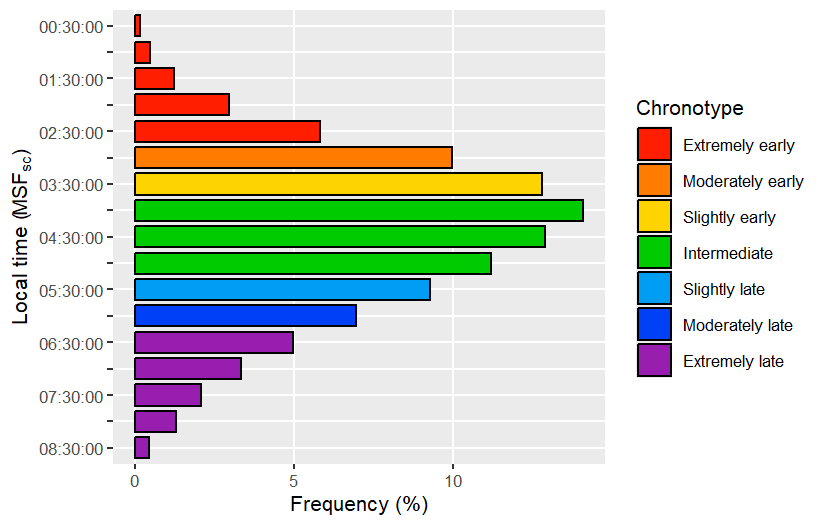
\includegraphics{qmd/chapter-5_files/figure-pdf/unnamed-chunk-4-1.png}

\legend{Source: Created by the author. Based on data visualization found
in \textcite{roenneberg2019b}.}

}

\end{figure}%

The MSF\textsubscript{sc} curve had a skewness of \(0.284\) and a
kurtosis of \(2.773\). However, the distribution was not normal
accordingly to Kolmogorov-Smirnov test (\(\text{D} = 0.03717\);
\(\text{p-value} = 2e-16\)) and D'Agostino Skewness test
(\(\text{Z3} = 31.525\); \(\text{p-value} = 2.2e-16\))
\autocites[see][]{dagostino1990}[also][46, p.~101]{thode2002}.

A linear regression model was created with MSF\textsubscript{sc} as the
response variable and with age and sex as predictors
(\(\text{R}^{2} = 0.05373\); \(\text{F}(2, 76741) = 2180\),
\(\text{p-value} = 2e-16\)), the two most known predictors for
chronotype (\textcite{roenneberg2007a}). A Box-Cox transformation of the
response variable was needed to attend to the linear regression model
assumptions (\(\lambda = -1.1111\);
\(\text{MSF}_{\text{sc}}^{\lambda - 1} / \lambda\)). All coefficients
were significantly different than \(0\) (\(\text{p-value} = 2e-16\))
and, accordingly to D'Agostino Skewness test, the residuals were normal
(\(\text{Z3} = -1.1906\); \(\text{p-value} = 0.23383\)). Residual
homoscedasticity was verified by a Score Test for Heteroskedasticity
(\(\chi^{2} = 0.00\); \(\text{p-value} = 1\)). No collinearity was found
between the predictor variables (variance inflation factor:
\(\text{age} = 1.0012\); \(\text{sex} = 1.0012\)).

Another model was created on top of the first one, adding the latitude
as a predictor variable (\(\text{R}^{2} = 0.060698\);
\(\text{F}(3, 76740) = 1650\), \(\text{p-value} = 2e-16\)). All
coefficients were significantly different than 0
(\(\text{p-value} = 2e-16\)) and the residuals were normally distributed
accordingly to the D'Agostino Skewness test, (\(\text{Z3} = 0.0742\);
\(\text{p-value} = 0.94085\)). Residual homoscedasticity was verified by
a Score Test for Heteroskedasticity (\(\chi^{2} = 0.00\);
\(\text{p-value} = 1\)). No collinearity was found between the predictor
variables (variance inflation factor: \(\text{age} = 1.0065\);
\(\text{sex} = 1.0016\); \(\text{latitude} = 1.0056\)). The longitude
was not used as a predictor because it presented colinearity with the
latitude variable.

An \(\text{F}\) test for nested models showed a significant reduction of
the residual sum of squares (\(\text{F}(1, 76740) = 568.94\),
\(\text{p-value} = 2e-16\)), meaning that the latitude seems to produce
an effect on the chronotype. However, when estimating Cohen's \(f^2\)
effect size, the result was negligible \autocite{cohen1992}
\(((0.06069 - 0.05373) / (1 - 0.06069) = 0.00740\)).

\subsection{Discussion}\label{discussion}

It's important to note that a causal and linear relationship between
latitude and chronotype is an \emph{a priori} assumption. The objective
of this study is to test or falsify this hypothesis.

For the latitude hypothesis to be true, there must be a significant
association between these two variables when the most common covariates
are controlled. Predictive models, in this case, are an adequate method
for testing this.

The results show that even with a wide latitudinal spectrum and with a
big and aligned sample of biological states the latitude effect does not
reveal itself in a non-negligible size. Several studies indicate the
existence of this effect on the chronotype
\autocite{hut2013,leocadio-miguel2017,pittendrigh1991,randler2008,randler2017,roenneberg2003},
but, at this time, at least in humans, no empirical evidence can support
this claim. Our results are very similar to Leocadio-Miguel et al.
\autocite*{leocadio-miguel2017}, which also found a negligible effect
size (Cohen's \(f^{2} = 0.004143174\)). The inconsistency of the
latitude effect can be visualized in
Figure~\ref{fig-chapter-5-chronotype-distribution-by-latitude}.

\begin{figure}[H]

\caption{\label{fig-chapter-5-chronotype-distribution-by-latitude}Distribution
of mean aggregates of the local time of the sleep corrected midpoint
between sleep onset and sleep end on work-free days
(MSF\textsubscript{sc}), MCTQ proxy for measuring the chronotype, in
relation to latitude decimal degree intervals. Higher values of
MSF\textsubscript{sc} indicate a tendency toward a late chronotype. The
red line represents a linear regression, and the shaded area indicates a
pointwise 95\% confidence interval.}

\centering{

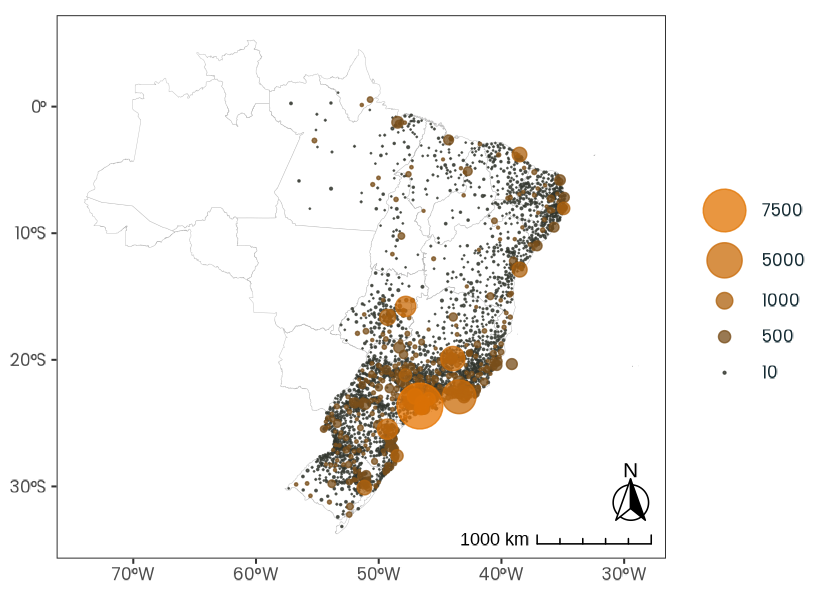
\includegraphics{qmd/chapter-5_files/figure-pdf/unnamed-chunk-5-1.png}

\legend{Source: Created by the author. Based on data visualization found
in \textcite{leocadio-miguel2017}.}

}

\end{figure}%

Despite the lack of evidence, is not uncommon to hear talks insisting
that this effect is real and already confirmed. We suspect that this
behavior may be derived from a lack of understanding of statistical
models and techniques. Although it may be logical and aligned with the
overall theory for the evolution of biological temporal systems, it's
our role as scientists to eliminate contractions, not pursue them.

The absence of a strong entrainment with the solar zeitgeber shows that
the entrainment phenomenon is more complex than we previously imagined.
Other hypotheses for the human circadian entrainment, like the
entrainment to self-selected light, proposed by Anna Skeldon and
Derk-Jan Dijk \autocite*{skeldon2021}, need to be tested and may produce
significant results. Methods and techiniques for complex systems, like
causal loop diagrams and agent-based models (ABM), may help to unravel
this phenomenon more properly.

It's important to notice that the results shown here are preliminary.
The data still needs some cleaning and to be balanced with Brazil's
latest population census. The latitude coordinates used in the analysis
are related to subjects' residential state capital and, hence, have low
resolution. Even with these results, it may be that a significant
latitude effect can still appear at the end of the research.

Despite the several strengths that the dataset used in this study has,
it is also important to notice its weaknesses and limitations. The fact
that all the subjects were measured in the Spring season is one of them.
Since the objective is to catch individuals in different seasonal
patterns, the ideal moment to collect this kind of data is in the
wintertime, when there is a greater insolation gradient between the
equator and the poles. Another one is that this dataset can be
influenced by the presence of a Daylight Saving Time (DST) event. This
latter issue is explored in more detail in the methods section.

\section{Methods}\label{methods}

\subsection{Measurement instrument}\label{measurement-instrument}

Chronotypes were measured using the core version of the standard Munich
ChronoType Questionnaire (MCTQ) \autocite{roenneberg2003}. MCTQ is a
widely validated and widely used self-report questionnaire for measuring
the sleep-wake cycle and chronotypes \autocite{roenneberg2019}. It
quantifies the chronotype as a state, a biological circadian phenotype,
using as a proxy the local time of the sleep corrected midpoint between
sleep onset and sleep end on work-free days (MSF\textsubscript{sc}). A
sleep correction (SC) is made when a possible sleep compensation related
to a lack of sleep on workdays is identified \autocite{roenneberg2012}.

Subjects were asked to complete an online questionnaire based on the
MCTQ Portuguese translation created by Till Roenneberg \& Martha Merrow
for the EUCLOCK project \autocite{roenneberg2006}
(\(\text{statements mean cosine distance} = 0.921\)). They were also
asked to provide sociodemographic (e.g., age, sex), geographic (e.g.,
full residential address), anthropometric (e.g., weight, height), and
work/study routine-related data. A deactivated version of the
questionnaire can be seen at \url{https://bit.ly/brchrono-form}.

\subsection{Sample}\label{sample}

The sample is made up of \(76,744\) Brazilian subjects. It was obtained
in 2017 from October 15th to 21st by a broadcast of the online
questionnaire on a popular Sunday TV show with national reach
\autocite{redeglobo2017}. This amount of data collected in such a short
time gave the sample a population cross-sectional characteristic.

A survey conducted in 2019 by the Brazilian Institute of Geography and
Statistics (IBGE) \autocite*{ibge2021} found that \(82.17\%\) of
Brazilian households had access to an internet connection. Therefore,
this sample is likely to have a good representation of Brazil's
population. Only residents of Brazilian states in the UTC-3 timezone,
aged \(18\) years or older, were included in the final sample.

In order to verify if the sample size was adequate for the study of the
phenomenon under investigation, a power analysis was conducted for
nested multiple regression models using the G*Power software
\autocite{faul2007}. The analysis used the parameters presented in
Leocadio-Miguel et al. \autocite*{leocadio-miguel2017} article for a
multiple linear regression with 10 tested predictors and only \(10\)
conceived predictors, considering a significance level of \(0.05\)
(\(\alpha\)) and a power of \(0.95\) (\(1 - \beta\)). The result showed
that a sample of \(5,895\) individuals would be necessary to test the
hypothesis.

Daylight Saving Time (DST) began in Brazil at midnight on October 15th,
2017. Residents from the Midwest, Southeast, and South regions were
instructed to set the clock forward by 1 hour. We believe that this
event did not contaminate the data since it started on the same day of
the data collection. It's important to notice that MCTQ asks subjects to
relate their routine behavior, not how they behaved in the last few
days. A possible effect of the DST on the sample is the production of an
even later chronotype for populations near the planet's poles,
amplifying a possible latitude effect. However, this was not shown on
the hypothesis test.

Based on the 2022 census \autocite{ibgea}, Brazil had \(52.263\%\) of
females and \(47.737\%\) of males with an age equal to or greater than
18 years old. The sample is skewed for female subjects, with
\(66.297\%\) of females and \(33.703\%\) of male subjects.

The subjects' mean age is \(32.015\) years (\(\text{SD} = 9.252\);
\(\text{Max.} = 58.786\)). Female subjects have a mean age of \(31.787\)
years (\(\text{SD} = 9.364\); \(\text{Max.} = 58.786\)) and male
subjects \(32.464\) years (\(\text{SD} = 9.012\);
\(\text{Max.} = 58.772\)). For comparison, based on the 2022 census
\autocite{ibgeb}, Brazil's population with an age equal to or greater
than \(18\) years old had a mean age of \(44.277\) years
(\(\text{SD} = 17.221\)), with a mean age of \(44.987\) years
(\(\text{SD} = 17.511\)) for female subjects and a mean age of
\(43.499\) years (\(\text{SD} = 16.864\)) for male subjects.

Considering the five regions of Brazil, the sample is mostly skewed for
the Southeast, the most populated region. According to Brazil's 2022
census \autocite{ibge2022}, the Southeast region is home to \(41.784\%\)
of Brazil's population, followed by the Northeast (\(26.910\%\)), South
(\(14.741\%\)), North (\(8.544\%\)), and Midwest (\(8.021\%\)) regions.
\(62.454\%\) of the sample is located in the Southeast region,
\(11.797\%\) in the Northeast, \(17.861\%\) in the South, \(1.682\%\) in
the North, and \(6.205\%\) in the Midwest region. Note that a lack of
subjects in the North and Midwest region is justified by the sample
timezone inclusion criteria (UTC-3).

The sample latitudinal range was \(30.211\) decimal degrees
(\(\text{Min.} = -30.109\); \(\text{Max.} = 0.10177\)) with a
longitudinal span of \(16.378\) decimal degrees
(\(\text{Min.} = -51.342\); \(\text{Max.} = -34.964\)). For comparison,
Brazil has a latitudinal range of \(39.024\) decimal degrees
(\(\text{Min.} = -33.752\); \(\text{Max.} = 5.2719\)) and a longitudinal
span of \(39.198\) decimal degrees (\(\text{Min.} = -34.793\);
\(\text{Max.} = -73.991\)).

\textbf{The results shown in this article are just a preliminary view of
the data analysis}. The latitudes and longitudes of each subject are
represented by the coordinates of his/her state's capital (a low
resolution). The final results will have the latitude and longitude
coordinates based on subjects' postal codes and will also use a balanced
dataset following the latest Brazil census.

\subsection{Data wrangling}\label{data-wrangling}

The data wrangling and analysis followed the data science program
proposed by Hadley Wickham and Garrett Grolemund \autocite{wickham2016}.
All processes were made with the help of the R programming language
\autocite{rcoreteam}, RStudio IDE \autocite{positteam}, and several R
packages. The tidyverse and rOpenSci package ecosystem and other R
packages adherents of the tidy tools manifesto \autocite{wickham2023a}
were prioritized. The MCTQ data was analyzed using the \texttt{mctq}
rOpenSci peer-reviewed package \autocite{vartanian2023}. All processes
were made in order to provide result reproducibility and to be in
accordance with the FAIR principles \autocite{wilkinson2016}.

\subsection{Hypothesis testing}\label{hypothesis-testing}

The study hypothesis was tested using nested models of multiple linear
regressions. The main idea of nested models is to verify the effect of
the inclusion of one or more predictors in the model variance
explanation (i.e., the \(\text{R}^{2}\)) \autocite{allen1997}. This can
be made by creating a restricted model and then comparing it with a full
model. Hence, the hypothesis can be schematized as follows.

\[
\begin{cases}
\text{H}_{0}: \Delta \ \text{Adjusted} \ \text{R}^{2} \leq \text{MES} \quad \text{or} \quad \text{F-test is not significant} \\
\text{H}_{a}: \Delta \ \text{Adjusted} \ \text{R}^{2} > \text{MES} \quad \text{and} \quad \text{F-test is significant}
\end{cases}
\]

\smallskip

In order to test a possible latitude association in predicting the
chronotype, the full model was the restricted model with the addition of
the latitude variable. The restricted model had the local time of the
sleep corrected midpoint between sleep onset and sleep end on work-free
days (MSF\textsubscript{sc}) as the response variable, MCTQ proxy for
the chronotype, with sex and age as predictors.

A residual analysis was made to ensure the validity of the models before
the hypothesis test. The hypothesis was tested using a \(0.05\)
(\(\alpha\)) significance level.

To favor the alternative hypothesis (\(\text{H}_{a}\)), not only the
\(\text{R}^{2}\) of the full model must be significantly larger than the
\(\text{R}^{2}\) of the restricted model, but the effect size must be at
least considered small. To evaluate the effect size, Cohen's \(f^{2}\)
and his categorical parameters for size were used \autocite{cohen1992}.
That means that, in order to favor (\(\text{H}_{a}\)), the effect size
must be at least equal to or greater than \(0.0219\).

\subsection{Data availability}\label{data-availability}

The data that support the findings of this study are available from the
corresponding author {[}DV{]}. Restrictions apply to the availability of
these data, which were used under the approval of a Research Ethics
Committee (REC) linked to the
\href{https://conselho.saude.gov.br/Web_comissoes/conep/index.html}{Brazilian
National Research Ethics Committee (CONEP)}, hence it cannot be publicly
shared. Data are, however, available from the author upon reasonable
request and with CONEP approval.

\subsection{Code availability}\label{code-availability}

The research compendium of the project is available under the
\href{https://opensource.org/license/mit/}{MIT license} at
\url{https://github.com/danielvartan/mastersthesis}. The code has all
the steps from the raw data to the test results.

\section{Acknowledgments}\label{acknowledgments}

Financial support was provided by the
\href{https://www.gov.br/capes/}{Coordination for the Improvement of
Higher Education Personnel (CAPES)} (Grant number:
88887.703720/2022-00).

\section{Ethics declarations}\label{ethics-declarations}

\subsection{Competing interests}\label{competing-interests}

The author declares that the study was carried out without any
commercial or financial connections that could be seen as a possible
competing interest.

\section{Additional information}\label{additional-information}

\textbf{This manuscript shows only preliminary results and should not be
considered as a document ready for journal submission.}

See the appendices section for supplementary information.

Correspondence can be sent to Daniel Vartanian
(\href{mailto:danvartan@gmail.com}{\nolinkurl{danvartan@gmail.com}}).

\section{Rights and permissions}\label{rights-and-permissions}

This article is released under the
\href{http://creativecommons.org/licenses/by/4.0/}{Creative Commons
Attribution 4.0 International License}, which permits use, sharing,
adaptation, distribution, and reproduction in any medium or format, as
long as be given appropriate credit to the original author and the
source, provide a link to the Creative Commons license, and indicate if
changes were made.

\bookmarksetup{startatroot}

\chapter{Conclusion}\label{conclusion}

\begin{tcolorbox}[enhanced jigsaw, opacitybacktitle=0.6, titlerule=0mm, coltitle=black, bottomtitle=1mm, breakable, rightrule=.15mm, left=2mm, title=\textcolor{quarto-callout-important-color}{\faExclamation}\hspace{0.5em}{Important}, opacityback=0, colbacktitle=quarto-callout-important-color!10!white, toprule=.15mm, toptitle=1mm, leftrule=.75mm, colback=white, bottomrule=.15mm, arc=.35mm, colframe=quarto-callout-important-color-frame]

You are reading the work-in-progress of this thesis.

\microskip

This chapter is currently a dumping ground for ideas, and I don't
recommend reading it.

\end{tcolorbox}

Conclusions

Limitations

Future perspectives

Initially, the thesis project proposed a global modeling approach to the
phenomenon. This approach was maintained due to the scope of a master's
degree program. As can be seen from the results of this and other
studies, no non-negligible effect regarding latitude and chronotype was
identified. It is possible, however, that this phenomenon, if it exists,
could be observed through a local approach using an agent-based model.
This approach would allow the simulation of an environment where agents
have varying light exposure and considering their endogenous rhythms and
the phase-response curve of the circadian clock to light. The data from
this thesis could be used to calibrate validate the model.

\postextual

\begingroup
\renewcommand{\baselinestretch}{1}
\setcounter{footnote}{0}
\renewcommand{\thefootnote}{\fnsymbol{footnote}}
\printbibliography[heading=bibheading]
\endgroup

\tocskipone
\tocprintchapternonum
\addcontentsline{toc}{chapter}{\newbibname}



\end{document}
